\documentclass[twoside]{book}

% Packages required by doxygen
\usepackage{fixltx2e}
\usepackage{calc}
\usepackage{doxygen}
\usepackage[export]{adjustbox} % also loads graphicx
\usepackage{graphicx}
\usepackage[utf8]{inputenc}
\usepackage{makeidx}
\usepackage{multicol}
\usepackage{multirow}
\PassOptionsToPackage{warn}{textcomp}
\usepackage{textcomp}
\usepackage[nointegrals]{wasysym}
\usepackage[table]{xcolor}

% Font selection
\usepackage[T1]{fontenc}
\usepackage[scaled=.90]{helvet}
\usepackage{courier}
\usepackage{amssymb}
\usepackage{sectsty}
\renewcommand{\familydefault}{\sfdefault}
\allsectionsfont{%
  \fontseries{bc}\selectfont%
  \color{darkgray}%
}
\renewcommand{\DoxyLabelFont}{%
  \fontseries{bc}\selectfont%
  \color{darkgray}%
}
\newcommand{\+}{\discretionary{\mbox{\scriptsize$\hookleftarrow$}}{}{}}

% Page & text layout
\usepackage{geometry}
\geometry{%
  a4paper,%
  top=2.5cm,%
  bottom=2.5cm,%
  left=2.5cm,%
  right=2.5cm%
}
\tolerance=750
\hfuzz=15pt
\hbadness=750
\setlength{\emergencystretch}{15pt}
\setlength{\parindent}{0cm}
\setlength{\parskip}{3ex plus 2ex minus 2ex}
\makeatletter
\renewcommand{\paragraph}{%
  \@startsection{paragraph}{4}{0ex}{-1.0ex}{1.0ex}{%
    \normalfont\normalsize\bfseries\SS@parafont%
  }%
}
\renewcommand{\subparagraph}{%
  \@startsection{subparagraph}{5}{0ex}{-1.0ex}{1.0ex}{%
    \normalfont\normalsize\bfseries\SS@subparafont%
  }%
}
\makeatother

% Headers & footers
\usepackage{fancyhdr}
\pagestyle{fancyplain}
\fancyhead[LE]{\fancyplain{}{\bfseries\thepage}}
\fancyhead[CE]{\fancyplain{}{}}
\fancyhead[RE]{\fancyplain{}{\bfseries\leftmark}}
\fancyhead[LO]{\fancyplain{}{\bfseries\rightmark}}
\fancyhead[CO]{\fancyplain{}{}}
\fancyhead[RO]{\fancyplain{}{\bfseries\thepage}}
\fancyfoot[LE]{\fancyplain{}{}}
\fancyfoot[CE]{\fancyplain{}{}}
\fancyfoot[RE]{\fancyplain{}{\bfseries\scriptsize Generated by Doxygen }}
\fancyfoot[LO]{\fancyplain{}{\bfseries\scriptsize Generated by Doxygen }}
\fancyfoot[CO]{\fancyplain{}{}}
\fancyfoot[RO]{\fancyplain{}{}}
\renewcommand{\footrulewidth}{0.4pt}
\renewcommand{\chaptermark}[1]{%
  \markboth{#1}{}%
}
\renewcommand{\sectionmark}[1]{%
  \markright{\thesection\ #1}%
}

% Indices & bibliography
\usepackage{natbib}
\usepackage[titles]{tocloft}
\setcounter{tocdepth}{3}
\setcounter{secnumdepth}{5}
\makeindex

% Hyperlinks (required, but should be loaded last)
\usepackage{ifpdf}
\ifpdf
  \usepackage[pdftex,pagebackref=true]{hyperref}
\else
  \usepackage[ps2pdf,pagebackref=true]{hyperref}
\fi
\hypersetup{%
  colorlinks=true,%
  linkcolor=blue,%
  citecolor=blue,%
  unicode%
}

% Custom commands
\newcommand{\clearemptydoublepage}{%
  \newpage{\pagestyle{empty}\cleardoublepage}%
}

\usepackage{caption}
\captionsetup{labelsep=space,justification=centering,font={bf},singlelinecheck=off,skip=4pt,position=top}

%===== C O N T E N T S =====

\begin{document}

% Titlepage & ToC
\hypersetup{pageanchor=false,
             bookmarksnumbered=true,
             pdfencoding=unicode
            }
\pagenumbering{roman}
\begin{titlepage}
\vspace*{7cm}
\begin{center}%
{\Large Final Project }\\
\vspace*{1cm}
{\large Generated by Doxygen 1.8.11}\\
\end{center}
\end{titlepage}
\clearemptydoublepage
\tableofcontents
\clearemptydoublepage
\pagenumbering{arabic}
\hypersetup{pageanchor=true}

%--- Begin generated contents ---
\chapter{Class Index}
\section{Class List}
Here are the classes, structs, unions and interfaces with brief descriptions\+:\begin{DoxyCompactList}
\item\contentsline{section}{\hyperlink{unionaccelerometer__raw__data__t}{accelerometer\+\_\+raw\+\_\+data\+\_\+t} }{\pageref{unionaccelerometer__raw__data__t}}{}
\item\contentsline{section}{\hyperlink{unioncompass__raw__data__t}{compass\+\_\+raw\+\_\+data\+\_\+t} }{\pageref{unioncompass__raw__data__t}}{}
\item\contentsline{section}{\hyperlink{structi2c__dev}{i2c\+\_\+dev} }{\pageref{structi2c__dev}}{}
\item\contentsline{section}{\hyperlink{structstate__machine__t}{state\+\_\+machine\+\_\+t} }{\pageref{structstate__machine__t}}{}
\end{DoxyCompactList}

\chapter{File Index}
\section{File List}
Here is a list of all files with brief descriptions\+:\begin{DoxyCompactList}
\item\contentsline{section}{/home/alexandre/\+S\+E/\+S\+E2017.\+2/\+Final\+Project/include/\hyperlink{accelerometer_8h}{accelerometer.\+h} }{\pageref{accelerometer_8h}}{}
\item\contentsline{section}{/home/alexandre/\+S\+E/\+S\+E2017.\+2/\+Final\+Project/include/\hyperlink{button_8h}{button.\+h} }{\pageref{button_8h}}{}
\item\contentsline{section}{/home/alexandre/\+S\+E/\+S\+E2017.\+2/\+Final\+Project/include/\hyperlink{compass_8h}{compass.\+h} }{\pageref{compass_8h}}{}
\item\contentsline{section}{/home/alexandre/\+S\+E/\+S\+E2017.\+2/\+Final\+Project/include/\hyperlink{display_8h}{display.\+h} }{\pageref{display_8h}}{}
\item\contentsline{section}{/home/alexandre/\+S\+E/\+S\+E2017.\+2/\+Final\+Project/include/\hyperlink{i2c__device_8h}{i2c\+\_\+device.\+h} }{\pageref{i2c__device_8h}}{}
\item\contentsline{section}{/home/alexandre/\+S\+E/\+S\+E2017.\+2/\+Final\+Project/include/\hyperlink{i2c__util_8h}{i2c\+\_\+util.\+h} }{\pageref{i2c__util_8h}}{}
\item\contentsline{section}{/home/alexandre/\+S\+E/\+S\+E2017.\+2/\+Final\+Project/include/\hyperlink{state__machine_8h}{state\+\_\+machine.\+h} }{\pageref{state__machine_8h}}{}
\item\contentsline{section}{/home/alexandre/\+S\+E/\+S\+E2017.\+2/\+Final\+Project/include/\hyperlink{thermometer_8h}{thermometer.\+h} }{\pageref{thermometer_8h}}{}
\end{DoxyCompactList}

\chapter{Class Documentation}
\hypertarget{unionaccelerometer__raw__data}{}\section{accelerometer\+\_\+raw\+\_\+data Union Reference}
\label{unionaccelerometer__raw__data}\index{accelerometer\+\_\+raw\+\_\+data@{accelerometer\+\_\+raw\+\_\+data}}


{\ttfamily \#include $<$accelerometer.\+h$>$}

\subsection*{Public Attributes}
\begin{DoxyCompactItemize}
\item 
\begin{tabbing}
xx\=xx\=xx\=xx\=xx\=xx\=xx\=xx\=xx\=\kill
struct \{\\
\>int16\_t \hyperlink{unionaccelerometer__raw__data_abe5cbfe31d12ba368d2a5679b8195d5f}{x}\\
\>int16\_t \hyperlink{unionaccelerometer__raw__data_a4fd1e05861d56ec35b0562563d70e15f}{y}\\
\>int16\_t \hyperlink{unionaccelerometer__raw__data_a18caf4ddfec4b38993aae2ad5e62819e}{z}\\
\} \hyperlink{unionaccelerometer__raw__data_a308f41f8f6fe55c187825216937cc729}{axis}\\

\end{tabbing}\begin{DoxyCompactList}\small\item\em Raw data for the raw values of the accelerometer as 3 separate 16-\/bit values. \end{DoxyCompactList}\item 
uint16\+\_\+t \hyperlink{unionaccelerometer__raw__data_a0e8bfd8a99a6c123b9a3f4e766dc98e3}{data\+\_\+signed} \mbox{[}3\mbox{]}
\begin{DoxyCompactList}\small\item\em data\+\_\+signed \end{DoxyCompactList}\item 
uint8\+\_\+t \hyperlink{unionaccelerometer__raw__data_ad5506633cb7fb456ed9fccdf2cbe6e5b}{data\+\_\+raw} \mbox{[}6\mbox{]}
\begin{DoxyCompactList}\small\item\em data\+\_\+raw \end{DoxyCompactList}\end{DoxyCompactItemize}


\subsection{Member Data Documentation}
\index{accelerometer\+\_\+raw\+\_\+data@{accelerometer\+\_\+raw\+\_\+data}!axis@{axis}}
\index{axis@{axis}!accelerometer\+\_\+raw\+\_\+data@{accelerometer\+\_\+raw\+\_\+data}}
\subsubsection[{\texorpdfstring{axis}{axis}}]{\setlength{\rightskip}{0pt plus 5cm}struct \{ ... \}   accelerometer\+\_\+raw\+\_\+data\+::axis}\hypertarget{unionaccelerometer__raw__data_a308f41f8f6fe55c187825216937cc729}{}\label{unionaccelerometer__raw__data_a308f41f8f6fe55c187825216937cc729}


Raw data for the raw values of the accelerometer as 3 separate 16-\/bit values. 

\index{accelerometer\+\_\+raw\+\_\+data@{accelerometer\+\_\+raw\+\_\+data}!data\+\_\+raw@{data\+\_\+raw}}
\index{data\+\_\+raw@{data\+\_\+raw}!accelerometer\+\_\+raw\+\_\+data@{accelerometer\+\_\+raw\+\_\+data}}
\subsubsection[{\texorpdfstring{data\+\_\+raw}{data_raw}}]{\setlength{\rightskip}{0pt plus 5cm}uint8\+\_\+t accelerometer\+\_\+raw\+\_\+data\+::data\+\_\+raw\mbox{[}6\mbox{]}}\hypertarget{unionaccelerometer__raw__data_ad5506633cb7fb456ed9fccdf2cbe6e5b}{}\label{unionaccelerometer__raw__data_ad5506633cb7fb456ed9fccdf2cbe6e5b}


data\+\_\+raw 

Raw data for the raw values of the accelerometer with each value separated in two 8-\/bit integer, as it is read from the device \index{accelerometer\+\_\+raw\+\_\+data@{accelerometer\+\_\+raw\+\_\+data}!data\+\_\+signed@{data\+\_\+signed}}
\index{data\+\_\+signed@{data\+\_\+signed}!accelerometer\+\_\+raw\+\_\+data@{accelerometer\+\_\+raw\+\_\+data}}
\subsubsection[{\texorpdfstring{data\+\_\+signed}{data_signed}}]{\setlength{\rightskip}{0pt plus 5cm}uint16\+\_\+t accelerometer\+\_\+raw\+\_\+data\+::data\+\_\+signed\mbox{[}3\mbox{]}}\hypertarget{unionaccelerometer__raw__data_a0e8bfd8a99a6c123b9a3f4e766dc98e3}{}\label{unionaccelerometer__raw__data_a0e8bfd8a99a6c123b9a3f4e766dc98e3}


data\+\_\+signed 

Raw data for the raw values of the accelerometer as a 16-\/bit array \index{accelerometer\+\_\+raw\+\_\+data@{accelerometer\+\_\+raw\+\_\+data}!x@{x}}
\index{x@{x}!accelerometer\+\_\+raw\+\_\+data@{accelerometer\+\_\+raw\+\_\+data}}
\subsubsection[{\texorpdfstring{x}{x}}]{\setlength{\rightskip}{0pt plus 5cm}int16\+\_\+t accelerometer\+\_\+raw\+\_\+data\+::x}\hypertarget{unionaccelerometer__raw__data_abe5cbfe31d12ba368d2a5679b8195d5f}{}\label{unionaccelerometer__raw__data_abe5cbfe31d12ba368d2a5679b8195d5f}
\index{accelerometer\+\_\+raw\+\_\+data@{accelerometer\+\_\+raw\+\_\+data}!y@{y}}
\index{y@{y}!accelerometer\+\_\+raw\+\_\+data@{accelerometer\+\_\+raw\+\_\+data}}
\subsubsection[{\texorpdfstring{y}{y}}]{\setlength{\rightskip}{0pt plus 5cm}int16\+\_\+t accelerometer\+\_\+raw\+\_\+data\+::y}\hypertarget{unionaccelerometer__raw__data_a4fd1e05861d56ec35b0562563d70e15f}{}\label{unionaccelerometer__raw__data_a4fd1e05861d56ec35b0562563d70e15f}
\index{accelerometer\+\_\+raw\+\_\+data@{accelerometer\+\_\+raw\+\_\+data}!z@{z}}
\index{z@{z}!accelerometer\+\_\+raw\+\_\+data@{accelerometer\+\_\+raw\+\_\+data}}
\subsubsection[{\texorpdfstring{z}{z}}]{\setlength{\rightskip}{0pt plus 5cm}int16\+\_\+t accelerometer\+\_\+raw\+\_\+data\+::z}\hypertarget{unionaccelerometer__raw__data_a18caf4ddfec4b38993aae2ad5e62819e}{}\label{unionaccelerometer__raw__data_a18caf4ddfec4b38993aae2ad5e62819e}


The documentation for this union was generated from the following file\+:\begin{DoxyCompactItemize}
\item 
/home/alexandre/\+S\+E/\+S\+E2017.\+2/\+Final\+Project/include/\hyperlink{accelerometer_8h}{accelerometer.\+h}\end{DoxyCompactItemize}

\hypertarget{unioncompass__raw__data}{}\section{compass\+\_\+raw\+\_\+data Union Reference}
\label{unioncompass__raw__data}\index{compass\+\_\+raw\+\_\+data@{compass\+\_\+raw\+\_\+data}}


{\ttfamily \#include $<$compass.\+h$>$}

\subsection*{Public Attributes}
\begin{DoxyCompactItemize}
\item 
\begin{tabbing}
xx\=xx\=xx\=xx\=xx\=xx\=xx\=xx\=xx\=\kill
struct \{\\
\>int16\_t \hyperlink{unioncompass__raw__data_abcb01e24cf0da22f4d89ea34b048e17c}{x}\\
\>int16\_t \hyperlink{unioncompass__raw__data_ab07fdca20a54692df8ff314d573c4313}{y}\\
\>int16\_t \hyperlink{unioncompass__raw__data_a489aa999829f2935717add753883667c}{z}\\
\} \hyperlink{unioncompass__raw__data_ae5fdba9f021adba1b201441884beee8f}{axis}\\

\end{tabbing}\item 
uint16\+\_\+t \hyperlink{unioncompass__raw__data_a597b0d6b3de62b99ee20496cc2919186}{data\+\_\+signed} \mbox{[}3\mbox{]}
\item 
uint8\+\_\+t \hyperlink{unioncompass__raw__data_a6e150d8de47f85ec9c6b0b3ef7c39f83}{data\+\_\+raw} \mbox{[}6\mbox{]}
\end{DoxyCompactItemize}


\subsection{Member Data Documentation}
\index{compass\+\_\+raw\+\_\+data@{compass\+\_\+raw\+\_\+data}!axis@{axis}}
\index{axis@{axis}!compass\+\_\+raw\+\_\+data@{compass\+\_\+raw\+\_\+data}}
\subsubsection[{\texorpdfstring{axis}{axis}}]{\setlength{\rightskip}{0pt plus 5cm}struct \{ ... \}   compass\+\_\+raw\+\_\+data\+::axis}\hypertarget{unioncompass__raw__data_ae5fdba9f021adba1b201441884beee8f}{}\label{unioncompass__raw__data_ae5fdba9f021adba1b201441884beee8f}
\index{compass\+\_\+raw\+\_\+data@{compass\+\_\+raw\+\_\+data}!data\+\_\+raw@{data\+\_\+raw}}
\index{data\+\_\+raw@{data\+\_\+raw}!compass\+\_\+raw\+\_\+data@{compass\+\_\+raw\+\_\+data}}
\subsubsection[{\texorpdfstring{data\+\_\+raw}{data_raw}}]{\setlength{\rightskip}{0pt plus 5cm}uint8\+\_\+t compass\+\_\+raw\+\_\+data\+::data\+\_\+raw\mbox{[}6\mbox{]}}\hypertarget{unioncompass__raw__data_a6e150d8de47f85ec9c6b0b3ef7c39f83}{}\label{unioncompass__raw__data_a6e150d8de47f85ec9c6b0b3ef7c39f83}
\index{compass\+\_\+raw\+\_\+data@{compass\+\_\+raw\+\_\+data}!data\+\_\+signed@{data\+\_\+signed}}
\index{data\+\_\+signed@{data\+\_\+signed}!compass\+\_\+raw\+\_\+data@{compass\+\_\+raw\+\_\+data}}
\subsubsection[{\texorpdfstring{data\+\_\+signed}{data_signed}}]{\setlength{\rightskip}{0pt plus 5cm}uint16\+\_\+t compass\+\_\+raw\+\_\+data\+::data\+\_\+signed\mbox{[}3\mbox{]}}\hypertarget{unioncompass__raw__data_a597b0d6b3de62b99ee20496cc2919186}{}\label{unioncompass__raw__data_a597b0d6b3de62b99ee20496cc2919186}
\index{compass\+\_\+raw\+\_\+data@{compass\+\_\+raw\+\_\+data}!x@{x}}
\index{x@{x}!compass\+\_\+raw\+\_\+data@{compass\+\_\+raw\+\_\+data}}
\subsubsection[{\texorpdfstring{x}{x}}]{\setlength{\rightskip}{0pt plus 5cm}int16\+\_\+t compass\+\_\+raw\+\_\+data\+::x}\hypertarget{unioncompass__raw__data_abcb01e24cf0da22f4d89ea34b048e17c}{}\label{unioncompass__raw__data_abcb01e24cf0da22f4d89ea34b048e17c}
\index{compass\+\_\+raw\+\_\+data@{compass\+\_\+raw\+\_\+data}!y@{y}}
\index{y@{y}!compass\+\_\+raw\+\_\+data@{compass\+\_\+raw\+\_\+data}}
\subsubsection[{\texorpdfstring{y}{y}}]{\setlength{\rightskip}{0pt plus 5cm}int16\+\_\+t compass\+\_\+raw\+\_\+data\+::y}\hypertarget{unioncompass__raw__data_ab07fdca20a54692df8ff314d573c4313}{}\label{unioncompass__raw__data_ab07fdca20a54692df8ff314d573c4313}
\index{compass\+\_\+raw\+\_\+data@{compass\+\_\+raw\+\_\+data}!z@{z}}
\index{z@{z}!compass\+\_\+raw\+\_\+data@{compass\+\_\+raw\+\_\+data}}
\subsubsection[{\texorpdfstring{z}{z}}]{\setlength{\rightskip}{0pt plus 5cm}int16\+\_\+t compass\+\_\+raw\+\_\+data\+::z}\hypertarget{unioncompass__raw__data_a489aa999829f2935717add753883667c}{}\label{unioncompass__raw__data_a489aa999829f2935717add753883667c}


The documentation for this union was generated from the following file\+:\begin{DoxyCompactItemize}
\item 
/home/alexandre/\+S\+E/\+S\+E2017.\+2/\+Final\+Project/include/\hyperlink{compass_8h}{compass.\+h}\end{DoxyCompactItemize}

\hypertarget{structi2c__dev}{}\section{i2c\+\_\+dev Struct Reference}
\label{structi2c__dev}\index{i2c\+\_\+dev@{i2c\+\_\+dev}}


{\ttfamily \#include $<$i2c\+\_\+util.\+h$>$}

\subsection*{Public Attributes}
\begin{DoxyCompactItemize}
\item 
struct device $\ast$ \hyperlink{structi2c__dev_ac4b6ba60143ff90df0ddc847deed7499}{dev}
\item 
char \hyperlink{structi2c__dev_aa3e3ecd39bec0681b174122b4a5e91e5}{name} \mbox{[}\hyperlink{i2c__util_8h_a48e1e64a2a8c3e1e1df44760d2a73eaa}{I2\+C\+\_\+\+D\+E\+V\+I\+C\+E\+\_\+\+N\+A\+M\+E\+\_\+\+L\+E\+N\+G\+TH}\mbox{]}
\item 
u16\+\_\+t \hyperlink{structi2c__dev_ae9308c72bfb06fea21da16f47b4e679b}{addr}
\item 
u8\+\_\+t \hyperlink{structi2c__dev_a20bd6a8e30216a5866cfc70fec9a3203}{reg\+\_\+test}
\item 
u8\+\_\+t \hyperlink{structi2c__dev_a46e0fffcf23e10012b1f5afc774088e7}{reg\+\_\+test\+\_\+expected\+\_\+val}
\end{DoxyCompactItemize}


\subsection{Member Data Documentation}
\index{i2c\+\_\+dev@{i2c\+\_\+dev}!addr@{addr}}
\index{addr@{addr}!i2c\+\_\+dev@{i2c\+\_\+dev}}
\subsubsection[{\texorpdfstring{addr}{addr}}]{\setlength{\rightskip}{0pt plus 5cm}u16\+\_\+t i2c\+\_\+dev\+::addr}\hypertarget{structi2c__dev_ae9308c72bfb06fea21da16f47b4e679b}{}\label{structi2c__dev_ae9308c72bfb06fea21da16f47b4e679b}
\index{i2c\+\_\+dev@{i2c\+\_\+dev}!dev@{dev}}
\index{dev@{dev}!i2c\+\_\+dev@{i2c\+\_\+dev}}
\subsubsection[{\texorpdfstring{dev}{dev}}]{\setlength{\rightskip}{0pt plus 5cm}struct device$\ast$ i2c\+\_\+dev\+::dev}\hypertarget{structi2c__dev_ac4b6ba60143ff90df0ddc847deed7499}{}\label{structi2c__dev_ac4b6ba60143ff90df0ddc847deed7499}
\index{i2c\+\_\+dev@{i2c\+\_\+dev}!name@{name}}
\index{name@{name}!i2c\+\_\+dev@{i2c\+\_\+dev}}
\subsubsection[{\texorpdfstring{name}{name}}]{\setlength{\rightskip}{0pt plus 5cm}char i2c\+\_\+dev\+::name\mbox{[}{\bf I2\+C\+\_\+\+D\+E\+V\+I\+C\+E\+\_\+\+N\+A\+M\+E\+\_\+\+L\+E\+N\+G\+TH}\mbox{]}}\hypertarget{structi2c__dev_aa3e3ecd39bec0681b174122b4a5e91e5}{}\label{structi2c__dev_aa3e3ecd39bec0681b174122b4a5e91e5}
\index{i2c\+\_\+dev@{i2c\+\_\+dev}!reg\+\_\+test@{reg\+\_\+test}}
\index{reg\+\_\+test@{reg\+\_\+test}!i2c\+\_\+dev@{i2c\+\_\+dev}}
\subsubsection[{\texorpdfstring{reg\+\_\+test}{reg_test}}]{\setlength{\rightskip}{0pt plus 5cm}u8\+\_\+t i2c\+\_\+dev\+::reg\+\_\+test}\hypertarget{structi2c__dev_a20bd6a8e30216a5866cfc70fec9a3203}{}\label{structi2c__dev_a20bd6a8e30216a5866cfc70fec9a3203}
\index{i2c\+\_\+dev@{i2c\+\_\+dev}!reg\+\_\+test\+\_\+expected\+\_\+val@{reg\+\_\+test\+\_\+expected\+\_\+val}}
\index{reg\+\_\+test\+\_\+expected\+\_\+val@{reg\+\_\+test\+\_\+expected\+\_\+val}!i2c\+\_\+dev@{i2c\+\_\+dev}}
\subsubsection[{\texorpdfstring{reg\+\_\+test\+\_\+expected\+\_\+val}{reg_test_expected_val}}]{\setlength{\rightskip}{0pt plus 5cm}u8\+\_\+t i2c\+\_\+dev\+::reg\+\_\+test\+\_\+expected\+\_\+val}\hypertarget{structi2c__dev_a46e0fffcf23e10012b1f5afc774088e7}{}\label{structi2c__dev_a46e0fffcf23e10012b1f5afc774088e7}


The documentation for this struct was generated from the following file\+:\begin{DoxyCompactItemize}
\item 
/home/alexandre/\+S\+E/\+S\+E2017.\+2/\+Final\+Project/include/\hyperlink{i2c__util_8h}{i2c\+\_\+util.\+h}\end{DoxyCompactItemize}

\hypertarget{structmstate__t}{}\section{mstate\+\_\+t Struct Reference}
\label{structmstate__t}\index{mstate\+\_\+t@{mstate\+\_\+t}}


{\ttfamily \#include $<$state\+\_\+machine.\+h$>$}

\subsection*{Public Attributes}
\begin{DoxyCompactItemize}
\item 
const char $\ast$ \hyperlink{structmstate__t_a4896c554397f6e870631cfa20181f5cb}{state\+\_\+name}
\item 
\hyperlink{state__machine_8h_aa0aafed44fec19806d8f9ad834be1248}{state\+\_\+t} \hyperlink{structmstate__t_ad7f00c99e78d768a8d426e35d90b57e9}{events} \mbox{[}2\mbox{]}
\item 
void($\ast$ \hyperlink{structmstate__t_a03f4847184c75e5655a23db334d31a7f}{action} )(void)
\end{DoxyCompactItemize}


\subsection{Member Data Documentation}
\index{mstate\+\_\+t@{mstate\+\_\+t}!action@{action}}
\index{action@{action}!mstate\+\_\+t@{mstate\+\_\+t}}
\subsubsection[{\texorpdfstring{action}{action}}]{\setlength{\rightskip}{0pt plus 5cm}void($\ast$ mstate\+\_\+t\+::action) (void)}\hypertarget{structmstate__t_a03f4847184c75e5655a23db334d31a7f}{}\label{structmstate__t_a03f4847184c75e5655a23db334d31a7f}
\index{mstate\+\_\+t@{mstate\+\_\+t}!events@{events}}
\index{events@{events}!mstate\+\_\+t@{mstate\+\_\+t}}
\subsubsection[{\texorpdfstring{events}{events}}]{\setlength{\rightskip}{0pt plus 5cm}{\bf state\+\_\+t} mstate\+\_\+t\+::events\mbox{[}2\mbox{]}}\hypertarget{structmstate__t_ad7f00c99e78d768a8d426e35d90b57e9}{}\label{structmstate__t_ad7f00c99e78d768a8d426e35d90b57e9}
\index{mstate\+\_\+t@{mstate\+\_\+t}!state\+\_\+name@{state\+\_\+name}}
\index{state\+\_\+name@{state\+\_\+name}!mstate\+\_\+t@{mstate\+\_\+t}}
\subsubsection[{\texorpdfstring{state\+\_\+name}{state_name}}]{\setlength{\rightskip}{0pt plus 5cm}const char$\ast$ mstate\+\_\+t\+::state\+\_\+name}\hypertarget{structmstate__t_a4896c554397f6e870631cfa20181f5cb}{}\label{structmstate__t_a4896c554397f6e870631cfa20181f5cb}


The documentation for this struct was generated from the following file\+:\begin{DoxyCompactItemize}
\item 
/home/alexandre/\+S\+E/\+S\+E2017.\+2/\+Final\+Project/include/\hyperlink{state__machine_8h}{state\+\_\+machine.\+h}\end{DoxyCompactItemize}

\chapter{File Documentation}
\hypertarget{accelerometer_8h}{}\section{/home/alexandre/\+S\+E/\+S\+E2017.2/\+Final\+Project/include/accelerometer.h File Reference}
\label{accelerometer_8h}\index{/home/alexandre/\+S\+E/\+S\+E2017.\+2/\+Final\+Project/include/accelerometer.\+h@{/home/alexandre/\+S\+E/\+S\+E2017.\+2/\+Final\+Project/include/accelerometer.\+h}}
{\ttfamily \#include \char`\"{}version.\+h\char`\"{}}\\*
{\ttfamily \#include \char`\"{}i2c\+\_\+device.\+h\char`\"{}}\\*
{\ttfamily \#include \char`\"{}display.\+h\char`\"{}}\\*
{\ttfamily \#include $<$stdint.\+h$>$}\\*
{\ttfamily \#include $<$math.\+h$>$}\\*
Include dependency graph for accelerometer.\+h\+:\nopagebreak
\begin{figure}[H]
\begin{center}
\leavevmode
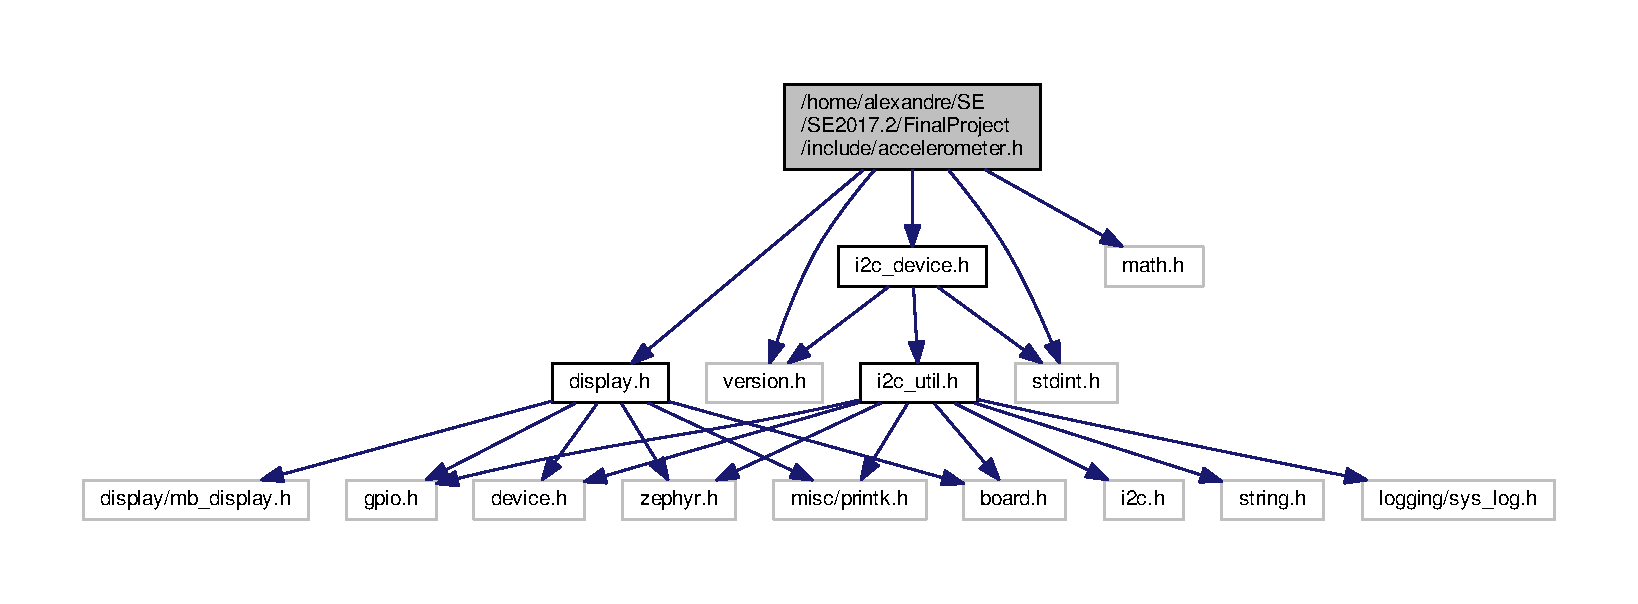
\includegraphics[width=350pt]{accelerometer_8h__incl}
\end{center}
\end{figure}
\subsection*{Classes}
\begin{DoxyCompactItemize}
\item 
union \hyperlink{unionaccelerometer__raw__data__t}{accelerometer\+\_\+raw\+\_\+data\+\_\+t}
\end{DoxyCompactItemize}
\subsection*{Macros}
\begin{DoxyCompactItemize}
\item 
\#define \hyperlink{accelerometer_8h_a6b05da58a833afa44a56889c577f0507}{A\+C\+C\+E\+L\+E\+R\+O\+M\+E\+T\+E\+R\+\_\+H}
\end{DoxyCompactItemize}
\subsection*{Functions}
\begin{DoxyCompactItemize}
\item 
static void \hyperlink{accelerometer_8h_a7c5c9cb545331e2bdd17cbb7c08ae1a0}{calculate\+\_\+tilt} (\hyperlink{unionaccelerometer__raw__data__t}{accelerometer\+\_\+raw\+\_\+data\+\_\+t} $\ast$data)
\begin{DoxyCompactList}\small\item\em calculate\+\_\+tilt Calculate roll and pitch of the device in degrees based on raw values \end{DoxyCompactList}\item 
void \hyperlink{accelerometer_8h_abdb57d2a6f27ead5805ff7956f699cc0}{show\+\_\+accelerometer} (void)
\begin{DoxyCompactList}\small\item\em print\+\_\+tilt Show current tilt as a pixel on the display \end{DoxyCompactList}\item 
static void \hyperlink{accelerometer_8h_ab18bf7ec3a3375958e1b46b43f872da7}{print\+\_\+tilt} (double\+\_\+t roll, double\+\_\+t pitch)
\begin{DoxyCompactList}\small\item\em show\+\_\+accelerometer Show current tilt as a pixel on the display \end{DoxyCompactList}\end{DoxyCompactItemize}


\subsection{Macro Definition Documentation}
\index{accelerometer.\+h@{accelerometer.\+h}!A\+C\+C\+E\+L\+E\+R\+O\+M\+E\+T\+E\+R\+\_\+H@{A\+C\+C\+E\+L\+E\+R\+O\+M\+E\+T\+E\+R\+\_\+H}}
\index{A\+C\+C\+E\+L\+E\+R\+O\+M\+E\+T\+E\+R\+\_\+H@{A\+C\+C\+E\+L\+E\+R\+O\+M\+E\+T\+E\+R\+\_\+H}!accelerometer.\+h@{accelerometer.\+h}}
\subsubsection[{\texorpdfstring{A\+C\+C\+E\+L\+E\+R\+O\+M\+E\+T\+E\+R\+\_\+H}{ACCELEROMETER_H}}]{\setlength{\rightskip}{0pt plus 5cm}\#define A\+C\+C\+E\+L\+E\+R\+O\+M\+E\+T\+E\+R\+\_\+H}\hypertarget{accelerometer_8h_a6b05da58a833afa44a56889c577f0507}{}\label{accelerometer_8h_a6b05da58a833afa44a56889c577f0507}


\subsection{Function Documentation}
\index{accelerometer.\+h@{accelerometer.\+h}!calculate\+\_\+tilt@{calculate\+\_\+tilt}}
\index{calculate\+\_\+tilt@{calculate\+\_\+tilt}!accelerometer.\+h@{accelerometer.\+h}}
\subsubsection[{\texorpdfstring{calculate\+\_\+tilt(accelerometer\+\_\+raw\+\_\+data\+\_\+t $\ast$data)}{calculate_tilt(accelerometer_raw_data_t *data)}}]{\setlength{\rightskip}{0pt plus 5cm}static void calculate\+\_\+tilt (
\begin{DoxyParamCaption}
\item[{{\bf accelerometer\+\_\+raw\+\_\+data\+\_\+t} $\ast$}]{data}
\end{DoxyParamCaption}
)\hspace{0.3cm}{\ttfamily [static]}}\hypertarget{accelerometer_8h_a7c5c9cb545331e2bdd17cbb7c08ae1a0}{}\label{accelerometer_8h_a7c5c9cb545331e2bdd17cbb7c08ae1a0}


calculate\+\_\+tilt Calculate roll and pitch of the device in degrees based on raw values 


\begin{DoxyParams}{Parameters}
{\em x\+\_\+raw} & -\/ raw x value \\
\hline
{\em y\+\_\+raw} & -\/ raw y value \\
\hline
{\em z\+\_\+raw} & -\/ raw z value \\
\hline
\end{DoxyParams}
\index{accelerometer.\+h@{accelerometer.\+h}!print\+\_\+tilt@{print\+\_\+tilt}}
\index{print\+\_\+tilt@{print\+\_\+tilt}!accelerometer.\+h@{accelerometer.\+h}}
\subsubsection[{\texorpdfstring{print\+\_\+tilt(double\+\_\+t roll, double\+\_\+t pitch)}{print_tilt(double_t roll, double_t pitch)}}]{\setlength{\rightskip}{0pt plus 5cm}static void print\+\_\+tilt (
\begin{DoxyParamCaption}
\item[{double\+\_\+t}]{roll, }
\item[{double\+\_\+t}]{pitch}
\end{DoxyParamCaption}
)\hspace{0.3cm}{\ttfamily [static]}}\hypertarget{accelerometer_8h_ab18bf7ec3a3375958e1b46b43f872da7}{}\label{accelerometer_8h_ab18bf7ec3a3375958e1b46b43f872da7}


show\+\_\+accelerometer Show current tilt as a pixel on the display 

\index{accelerometer.\+h@{accelerometer.\+h}!show\+\_\+accelerometer@{show\+\_\+accelerometer}}
\index{show\+\_\+accelerometer@{show\+\_\+accelerometer}!accelerometer.\+h@{accelerometer.\+h}}
\subsubsection[{\texorpdfstring{show\+\_\+accelerometer(void)}{show_accelerometer(void)}}]{\setlength{\rightskip}{0pt plus 5cm}void show\+\_\+accelerometer (
\begin{DoxyParamCaption}
\item[{void}]{}
\end{DoxyParamCaption}
)}\hypertarget{accelerometer_8h_abdb57d2a6f27ead5805ff7956f699cc0}{}\label{accelerometer_8h_abdb57d2a6f27ead5805ff7956f699cc0}


print\+\_\+tilt Show current tilt as a pixel on the display 


\begin{DoxyParams}{Parameters}
{\em roll} & -\/ roll of device \\
\hline
{\em pitch} & -\/ pitch of the device \\
\hline
\end{DoxyParams}

\hypertarget{button_8h}{}\section{/home/alexandre/\+S\+E/\+S\+E2017.2/\+Final\+Project/include/button.h File Reference}
\label{button_8h}\index{/home/alexandre/\+S\+E/\+S\+E2017.\+2/\+Final\+Project/include/button.\+h@{/home/alexandre/\+S\+E/\+S\+E2017.\+2/\+Final\+Project/include/button.\+h}}
{\ttfamily \#include $<$zephyr.\+h$>$}\\*
{\ttfamily \#include $<$board.\+h$>$}\\*
{\ttfamily \#include $<$device.\+h$>$}\\*
{\ttfamily \#include $<$gpio.\+h$>$}\\*
{\ttfamily \#include $<$misc/util.\+h$>$}\\*
{\ttfamily \#include $<$misc/printk.\+h$>$}\\*
Include dependency graph for button.\+h\+:\nopagebreak
\begin{figure}[H]
\begin{center}
\leavevmode
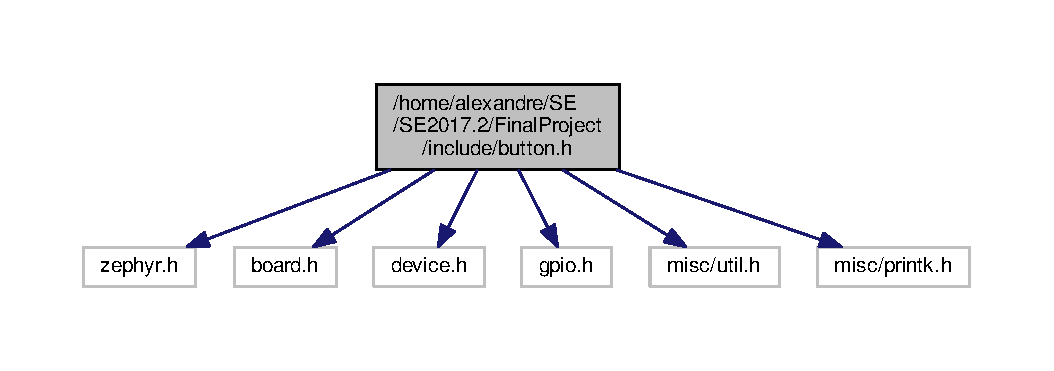
\includegraphics[width=350pt]{button_8h__incl}
\end{center}
\end{figure}
\subsection*{Macros}
\begin{DoxyCompactItemize}
\item 
\#define \hyperlink{button_8h_a4f41aabd288a68e43ce55ed0da4a9d9e}{E\+D\+G\+E0}~(G\+P\+I\+O\+\_\+\+I\+N\+T\+\_\+\+E\+D\+GE $\vert$ G\+P\+I\+O\+\_\+\+I\+N\+T\+\_\+\+A\+C\+T\+I\+V\+E\+\_\+\+L\+OW)
\item 
\#define \hyperlink{button_8h_a6219915dce04c118e709cb9b42995ace}{P\+U\+L\+L\+\_\+\+U\+P0}~0
\item 
\#define \hyperlink{button_8h_a7af108eb6da3fc4e6000d9a72a20090c}{E\+D\+G\+E1}~(G\+P\+I\+O\+\_\+\+I\+N\+T\+\_\+\+E\+D\+GE $\vert$ G\+P\+I\+O\+\_\+\+I\+N\+T\+\_\+\+A\+C\+T\+I\+V\+E\+\_\+\+L\+OW)
\item 
\#define \hyperlink{button_8h_af68bd9faf51a6ed2f123394d203c1609}{P\+U\+L\+L\+\_\+\+U\+P1}~0
\item 
\#define \hyperlink{button_8h_abe0b7b2a0ec4b64b92585808a051e1fa}{S\+L\+E\+E\+P\+\_\+\+T\+I\+ME}~500
\end{DoxyCompactItemize}
\subsection*{Functions}
\begin{DoxyCompactItemize}
\item 
void \hyperlink{button_8h_aa3c093a39a523c665a32edd75551c4ec}{button\+\_\+\+A\+\_\+set\+\_\+callback} (gpio\+\_\+callback\+\_\+handler\+\_\+t callback)
\begin{DoxyCompactList}\small\item\em button\+\_\+\+B\+\_\+set\+\_\+callback Sets a I\+SR to be called when button B is triggered \end{DoxyCompactList}\item 
void \hyperlink{button_8h_a6fd11c2b2f170bd2f39bdcd58b3c8093}{button\+\_\+\+B\+\_\+set\+\_\+callback} (gpio\+\_\+callback\+\_\+handler\+\_\+t callback)
\begin{DoxyCompactList}\small\item\em button\+\_\+\+A\+\_\+set\+\_\+callback Sets a I\+SR to be called when button A is triggered \end{DoxyCompactList}\item 
void \hyperlink{button_8h_a64a0f16b645b1f5205cbc27a267f8e63}{button\+\_\+configure\+\_\+init} (void)
\begin{DoxyCompactList}\small\item\em button\+\_\+configure\+\_\+init Configure ports for buttons A and B \end{DoxyCompactList}\end{DoxyCompactItemize}


\subsection{Macro Definition Documentation}
\index{button.\+h@{button.\+h}!E\+D\+G\+E0@{E\+D\+G\+E0}}
\index{E\+D\+G\+E0@{E\+D\+G\+E0}!button.\+h@{button.\+h}}
\subsubsection[{\texorpdfstring{E\+D\+G\+E0}{EDGE0}}]{\setlength{\rightskip}{0pt plus 5cm}\#define E\+D\+G\+E0~(G\+P\+I\+O\+\_\+\+I\+N\+T\+\_\+\+E\+D\+GE $\vert$ G\+P\+I\+O\+\_\+\+I\+N\+T\+\_\+\+A\+C\+T\+I\+V\+E\+\_\+\+L\+OW)}\hypertarget{button_8h_a4f41aabd288a68e43ce55ed0da4a9d9e}{}\label{button_8h_a4f41aabd288a68e43ce55ed0da4a9d9e}
\index{button.\+h@{button.\+h}!E\+D\+G\+E1@{E\+D\+G\+E1}}
\index{E\+D\+G\+E1@{E\+D\+G\+E1}!button.\+h@{button.\+h}}
\subsubsection[{\texorpdfstring{E\+D\+G\+E1}{EDGE1}}]{\setlength{\rightskip}{0pt plus 5cm}\#define E\+D\+G\+E1~(G\+P\+I\+O\+\_\+\+I\+N\+T\+\_\+\+E\+D\+GE $\vert$ G\+P\+I\+O\+\_\+\+I\+N\+T\+\_\+\+A\+C\+T\+I\+V\+E\+\_\+\+L\+OW)}\hypertarget{button_8h_a7af108eb6da3fc4e6000d9a72a20090c}{}\label{button_8h_a7af108eb6da3fc4e6000d9a72a20090c}
\index{button.\+h@{button.\+h}!P\+U\+L\+L\+\_\+\+U\+P0@{P\+U\+L\+L\+\_\+\+U\+P0}}
\index{P\+U\+L\+L\+\_\+\+U\+P0@{P\+U\+L\+L\+\_\+\+U\+P0}!button.\+h@{button.\+h}}
\subsubsection[{\texorpdfstring{P\+U\+L\+L\+\_\+\+U\+P0}{PULL_UP0}}]{\setlength{\rightskip}{0pt plus 5cm}\#define P\+U\+L\+L\+\_\+\+U\+P0~0}\hypertarget{button_8h_a6219915dce04c118e709cb9b42995ace}{}\label{button_8h_a6219915dce04c118e709cb9b42995ace}
\index{button.\+h@{button.\+h}!P\+U\+L\+L\+\_\+\+U\+P1@{P\+U\+L\+L\+\_\+\+U\+P1}}
\index{P\+U\+L\+L\+\_\+\+U\+P1@{P\+U\+L\+L\+\_\+\+U\+P1}!button.\+h@{button.\+h}}
\subsubsection[{\texorpdfstring{P\+U\+L\+L\+\_\+\+U\+P1}{PULL_UP1}}]{\setlength{\rightskip}{0pt plus 5cm}\#define P\+U\+L\+L\+\_\+\+U\+P1~0}\hypertarget{button_8h_af68bd9faf51a6ed2f123394d203c1609}{}\label{button_8h_af68bd9faf51a6ed2f123394d203c1609}
\index{button.\+h@{button.\+h}!S\+L\+E\+E\+P\+\_\+\+T\+I\+ME@{S\+L\+E\+E\+P\+\_\+\+T\+I\+ME}}
\index{S\+L\+E\+E\+P\+\_\+\+T\+I\+ME@{S\+L\+E\+E\+P\+\_\+\+T\+I\+ME}!button.\+h@{button.\+h}}
\subsubsection[{\texorpdfstring{S\+L\+E\+E\+P\+\_\+\+T\+I\+ME}{SLEEP_TIME}}]{\setlength{\rightskip}{0pt plus 5cm}\#define S\+L\+E\+E\+P\+\_\+\+T\+I\+ME~500}\hypertarget{button_8h_abe0b7b2a0ec4b64b92585808a051e1fa}{}\label{button_8h_abe0b7b2a0ec4b64b92585808a051e1fa}


\subsection{Function Documentation}
\index{button.\+h@{button.\+h}!button\+\_\+\+A\+\_\+set\+\_\+callback@{button\+\_\+\+A\+\_\+set\+\_\+callback}}
\index{button\+\_\+\+A\+\_\+set\+\_\+callback@{button\+\_\+\+A\+\_\+set\+\_\+callback}!button.\+h@{button.\+h}}
\subsubsection[{\texorpdfstring{button\+\_\+\+A\+\_\+set\+\_\+callback(gpio\+\_\+callback\+\_\+handler\+\_\+t callback)}{button_A_set_callback(gpio_callback_handler_t callback)}}]{\setlength{\rightskip}{0pt plus 5cm}void button\+\_\+\+A\+\_\+set\+\_\+callback (
\begin{DoxyParamCaption}
\item[{gpio\+\_\+callback\+\_\+handler\+\_\+t}]{callback}
\end{DoxyParamCaption}
)}\hypertarget{button_8h_aa3c093a39a523c665a32edd75551c4ec}{}\label{button_8h_aa3c093a39a523c665a32edd75551c4ec}


button\+\_\+\+B\+\_\+set\+\_\+callback Sets a I\+SR to be called when button B is triggered 


\begin{DoxyParams}{Parameters}
{\em callback} & -\/ I\+SR to be called \\
\hline
\end{DoxyParams}
\index{button.\+h@{button.\+h}!button\+\_\+\+B\+\_\+set\+\_\+callback@{button\+\_\+\+B\+\_\+set\+\_\+callback}}
\index{button\+\_\+\+B\+\_\+set\+\_\+callback@{button\+\_\+\+B\+\_\+set\+\_\+callback}!button.\+h@{button.\+h}}
\subsubsection[{\texorpdfstring{button\+\_\+\+B\+\_\+set\+\_\+callback(gpio\+\_\+callback\+\_\+handler\+\_\+t callback)}{button_B_set_callback(gpio_callback_handler_t callback)}}]{\setlength{\rightskip}{0pt plus 5cm}void button\+\_\+\+B\+\_\+set\+\_\+callback (
\begin{DoxyParamCaption}
\item[{gpio\+\_\+callback\+\_\+handler\+\_\+t}]{callback}
\end{DoxyParamCaption}
)}\hypertarget{button_8h_a6fd11c2b2f170bd2f39bdcd58b3c8093}{}\label{button_8h_a6fd11c2b2f170bd2f39bdcd58b3c8093}


button\+\_\+\+A\+\_\+set\+\_\+callback Sets a I\+SR to be called when button A is triggered 


\begin{DoxyParams}{Parameters}
{\em callback} & -\/ I\+SR to be called \\
\hline
\end{DoxyParams}
\index{button.\+h@{button.\+h}!button\+\_\+configure\+\_\+init@{button\+\_\+configure\+\_\+init}}
\index{button\+\_\+configure\+\_\+init@{button\+\_\+configure\+\_\+init}!button.\+h@{button.\+h}}
\subsubsection[{\texorpdfstring{button\+\_\+configure\+\_\+init(void)}{button_configure_init(void)}}]{\setlength{\rightskip}{0pt plus 5cm}void button\+\_\+configure\+\_\+init (
\begin{DoxyParamCaption}
\item[{void}]{}
\end{DoxyParamCaption}
)}\hypertarget{button_8h_a64a0f16b645b1f5205cbc27a267f8e63}{}\label{button_8h_a64a0f16b645b1f5205cbc27a267f8e63}


button\+\_\+configure\+\_\+init Configure ports for buttons A and B 


\hypertarget{compass_8h}{}\section{/home/alexandre/\+S\+E/\+S\+E2017.2/\+Final\+Project/include/compass.h File Reference}
\label{compass_8h}\index{/home/alexandre/\+S\+E/\+S\+E2017.\+2/\+Final\+Project/include/compass.\+h@{/home/alexandre/\+S\+E/\+S\+E2017.\+2/\+Final\+Project/include/compass.\+h}}
{\ttfamily \#include $<$stdint.\+h$>$}\\*
{\ttfamily \#include \char`\"{}math.\+h\char`\"{}}\\*
{\ttfamily \#include \char`\"{}display.\+h\char`\"{}}\\*
{\ttfamily \#include $<$misc/printk.\+h$>$}\\*
{\ttfamily \#include \char`\"{}version.\+h\char`\"{}}\\*
{\ttfamily \#include \char`\"{}i2c\+\_\+util.\+h\char`\"{}}\\*
Include dependency graph for compass.\+h\+:\nopagebreak
\begin{figure}[H]
\begin{center}
\leavevmode
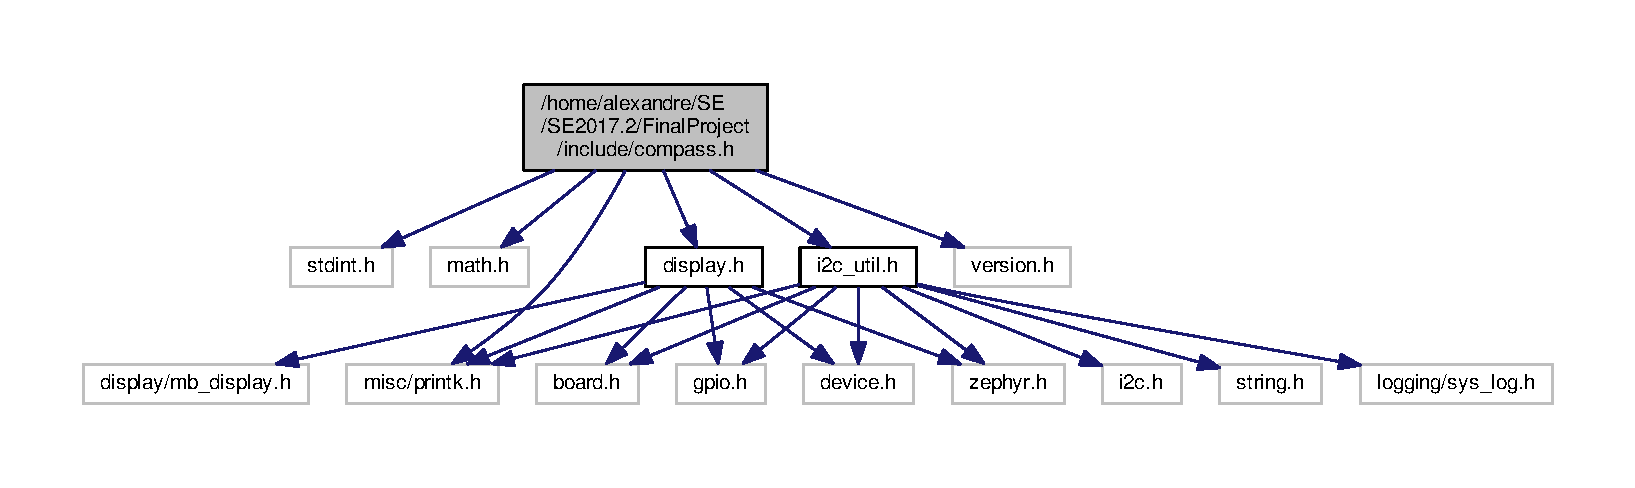
\includegraphics[width=350pt]{compass_8h__incl}
\end{center}
\end{figure}
\subsection*{Classes}
\begin{DoxyCompactItemize}
\item 
union \hyperlink{unioncompass__raw__data__t}{compass\+\_\+raw\+\_\+data\+\_\+t}
\end{DoxyCompactItemize}
\subsection*{Enumerations}
\begin{DoxyCompactItemize}
\item 
enum \hyperlink{compass_8h_ae9ae980041e438eed7a3af43ce4e9f6b}{direction\+\_\+t} \{ \\*
\hyperlink{compass_8h_ae9ae980041e438eed7a3af43ce4e9f6bad0611de6f28d4a9c9eac959f5344698e}{N\+O\+R\+TH}, 
\hyperlink{compass_8h_ae9ae980041e438eed7a3af43ce4e9f6bae9449e8683a8199dad36b07a63b2f523}{W\+E\+ST}, 
\hyperlink{compass_8h_ae9ae980041e438eed7a3af43ce4e9f6ba8ef5c0bce69283a9986011a63eea8a6b}{S\+O\+U\+TH}, 
\hyperlink{compass_8h_ae9ae980041e438eed7a3af43ce4e9f6bab5b3793b961949c817c7c0d99c05dad7}{E\+A\+ST}, 
\\*
\hyperlink{compass_8h_ae9ae980041e438eed7a3af43ce4e9f6bac8aee466c121a3c3c942f58e1d8864d4}{N\+O\+R\+T\+H\+W\+E\+ST}, 
\hyperlink{compass_8h_ae9ae980041e438eed7a3af43ce4e9f6ba46b2b49ffff37706df1f1497d31a458c}{N\+O\+R\+T\+H\+T\+E\+A\+ST}, 
\hyperlink{compass_8h_ae9ae980041e438eed7a3af43ce4e9f6ba6aa90951b336be999de204e61dd366d4}{S\+O\+U\+T\+H\+W\+E\+ST}, 
\hyperlink{compass_8h_ae9ae980041e438eed7a3af43ce4e9f6ba16c2c7abfbd3bad3343b0dcaa858bb49}{S\+O\+U\+T\+H\+E\+A\+ST}, 
\\*
\hyperlink{compass_8h_ae9ae980041e438eed7a3af43ce4e9f6ba605159e8a4c32319fd69b5d151369d93}{U\+N\+D\+E\+F\+I\+N\+ED}
 \}
\end{DoxyCompactItemize}
\subsection*{Functions}
\begin{DoxyCompactItemize}
\item 
\hyperlink{compass_8h_ae9ae980041e438eed7a3af43ce4e9f6b}{direction\+\_\+t} \hyperlink{compass_8h_a709e55d460e36e7126d379ebf2080c22}{calculate\+\_\+direction} (\hyperlink{unioncompass__raw__data__t}{compass\+\_\+raw\+\_\+data\+\_\+t} $\ast$data)
\begin{DoxyCompactList}\small\item\em calculate\+\_\+direction \end{DoxyCompactList}\item 
void \hyperlink{compass_8h_ae937ab674d54bc076783f8206002be7f}{show\+\_\+compass} (void)
\begin{DoxyCompactList}\small\item\em show\+\_\+compass Show direction of magnetic north on the display \end{DoxyCompactList}\item 
struct mb\+\_\+display $\ast$ \hyperlink{compass_8h_a0fc6682575beba29c58f3b86289c35c8}{compass\+\_\+direction\+\_\+sprite\+\_\+get} (\hyperlink{compass_8h_ae9ae980041e438eed7a3af43ce4e9f6b}{direction\+\_\+t} direction)
\begin{DoxyCompactList}\small\item\em compass\+\_\+direction\+\_\+sprite\+\_\+get Get the sprite for a cardinal direction to be shown on the display \end{DoxyCompactList}\end{DoxyCompactItemize}


\subsection{Enumeration Type Documentation}
\index{compass.\+h@{compass.\+h}!direction\+\_\+t@{direction\+\_\+t}}
\index{direction\+\_\+t@{direction\+\_\+t}!compass.\+h@{compass.\+h}}
\subsubsection[{\texorpdfstring{direction\+\_\+t}{direction_t}}]{\setlength{\rightskip}{0pt plus 5cm}enum {\bf direction\+\_\+t}}\hypertarget{compass_8h_ae9ae980041e438eed7a3af43ce4e9f6b}{}\label{compass_8h_ae9ae980041e438eed7a3af43ce4e9f6b}
\begin{Desc}
\item[Enumerator]\par
\begin{description}
\index{N\+O\+R\+TH@{N\+O\+R\+TH}!compass.\+h@{compass.\+h}}\index{compass.\+h@{compass.\+h}!N\+O\+R\+TH@{N\+O\+R\+TH}}\item[{\em 
N\+O\+R\+TH\hypertarget{compass_8h_ae9ae980041e438eed7a3af43ce4e9f6bad0611de6f28d4a9c9eac959f5344698e}{}\label{compass_8h_ae9ae980041e438eed7a3af43ce4e9f6bad0611de6f28d4a9c9eac959f5344698e}
}]\index{W\+E\+ST@{W\+E\+ST}!compass.\+h@{compass.\+h}}\index{compass.\+h@{compass.\+h}!W\+E\+ST@{W\+E\+ST}}\item[{\em 
W\+E\+ST\hypertarget{compass_8h_ae9ae980041e438eed7a3af43ce4e9f6bae9449e8683a8199dad36b07a63b2f523}{}\label{compass_8h_ae9ae980041e438eed7a3af43ce4e9f6bae9449e8683a8199dad36b07a63b2f523}
}]\index{S\+O\+U\+TH@{S\+O\+U\+TH}!compass.\+h@{compass.\+h}}\index{compass.\+h@{compass.\+h}!S\+O\+U\+TH@{S\+O\+U\+TH}}\item[{\em 
S\+O\+U\+TH\hypertarget{compass_8h_ae9ae980041e438eed7a3af43ce4e9f6ba8ef5c0bce69283a9986011a63eea8a6b}{}\label{compass_8h_ae9ae980041e438eed7a3af43ce4e9f6ba8ef5c0bce69283a9986011a63eea8a6b}
}]\index{E\+A\+ST@{E\+A\+ST}!compass.\+h@{compass.\+h}}\index{compass.\+h@{compass.\+h}!E\+A\+ST@{E\+A\+ST}}\item[{\em 
E\+A\+ST\hypertarget{compass_8h_ae9ae980041e438eed7a3af43ce4e9f6bab5b3793b961949c817c7c0d99c05dad7}{}\label{compass_8h_ae9ae980041e438eed7a3af43ce4e9f6bab5b3793b961949c817c7c0d99c05dad7}
}]\index{N\+O\+R\+T\+H\+W\+E\+ST@{N\+O\+R\+T\+H\+W\+E\+ST}!compass.\+h@{compass.\+h}}\index{compass.\+h@{compass.\+h}!N\+O\+R\+T\+H\+W\+E\+ST@{N\+O\+R\+T\+H\+W\+E\+ST}}\item[{\em 
N\+O\+R\+T\+H\+W\+E\+ST\hypertarget{compass_8h_ae9ae980041e438eed7a3af43ce4e9f6bac8aee466c121a3c3c942f58e1d8864d4}{}\label{compass_8h_ae9ae980041e438eed7a3af43ce4e9f6bac8aee466c121a3c3c942f58e1d8864d4}
}]\index{N\+O\+R\+T\+H\+T\+E\+A\+ST@{N\+O\+R\+T\+H\+T\+E\+A\+ST}!compass.\+h@{compass.\+h}}\index{compass.\+h@{compass.\+h}!N\+O\+R\+T\+H\+T\+E\+A\+ST@{N\+O\+R\+T\+H\+T\+E\+A\+ST}}\item[{\em 
N\+O\+R\+T\+H\+T\+E\+A\+ST\hypertarget{compass_8h_ae9ae980041e438eed7a3af43ce4e9f6ba46b2b49ffff37706df1f1497d31a458c}{}\label{compass_8h_ae9ae980041e438eed7a3af43ce4e9f6ba46b2b49ffff37706df1f1497d31a458c}
}]\index{S\+O\+U\+T\+H\+W\+E\+ST@{S\+O\+U\+T\+H\+W\+E\+ST}!compass.\+h@{compass.\+h}}\index{compass.\+h@{compass.\+h}!S\+O\+U\+T\+H\+W\+E\+ST@{S\+O\+U\+T\+H\+W\+E\+ST}}\item[{\em 
S\+O\+U\+T\+H\+W\+E\+ST\hypertarget{compass_8h_ae9ae980041e438eed7a3af43ce4e9f6ba6aa90951b336be999de204e61dd366d4}{}\label{compass_8h_ae9ae980041e438eed7a3af43ce4e9f6ba6aa90951b336be999de204e61dd366d4}
}]\index{S\+O\+U\+T\+H\+E\+A\+ST@{S\+O\+U\+T\+H\+E\+A\+ST}!compass.\+h@{compass.\+h}}\index{compass.\+h@{compass.\+h}!S\+O\+U\+T\+H\+E\+A\+ST@{S\+O\+U\+T\+H\+E\+A\+ST}}\item[{\em 
S\+O\+U\+T\+H\+E\+A\+ST\hypertarget{compass_8h_ae9ae980041e438eed7a3af43ce4e9f6ba16c2c7abfbd3bad3343b0dcaa858bb49}{}\label{compass_8h_ae9ae980041e438eed7a3af43ce4e9f6ba16c2c7abfbd3bad3343b0dcaa858bb49}
}]\index{U\+N\+D\+E\+F\+I\+N\+ED@{U\+N\+D\+E\+F\+I\+N\+ED}!compass.\+h@{compass.\+h}}\index{compass.\+h@{compass.\+h}!U\+N\+D\+E\+F\+I\+N\+ED@{U\+N\+D\+E\+F\+I\+N\+ED}}\item[{\em 
U\+N\+D\+E\+F\+I\+N\+ED\hypertarget{compass_8h_ae9ae980041e438eed7a3af43ce4e9f6ba605159e8a4c32319fd69b5d151369d93}{}\label{compass_8h_ae9ae980041e438eed7a3af43ce4e9f6ba605159e8a4c32319fd69b5d151369d93}
}]\end{description}
\end{Desc}


\subsection{Function Documentation}
\index{compass.\+h@{compass.\+h}!calculate\+\_\+direction@{calculate\+\_\+direction}}
\index{calculate\+\_\+direction@{calculate\+\_\+direction}!compass.\+h@{compass.\+h}}
\subsubsection[{\texorpdfstring{calculate\+\_\+direction(compass\+\_\+raw\+\_\+data\+\_\+t $\ast$data)}{calculate_direction(compass_raw_data_t *data)}}]{\setlength{\rightskip}{0pt plus 5cm}{\bf direction\+\_\+t} calculate\+\_\+direction (
\begin{DoxyParamCaption}
\item[{{\bf compass\+\_\+raw\+\_\+data\+\_\+t} $\ast$}]{data}
\end{DoxyParamCaption}
)}\hypertarget{compass_8h_a709e55d460e36e7126d379ebf2080c22}{}\label{compass_8h_a709e55d460e36e7126d379ebf2080c22}


calculate\+\_\+direction 

Calculate north direction based on raw magnetometer data


\begin{DoxyParams}{Parameters}
{\em data} & Raw magnetometer data\\
\hline
\end{DoxyParams}
\begin{DoxyReturn}{Returns}
The calculated cardinal direction 
\end{DoxyReturn}
\index{compass.\+h@{compass.\+h}!compass\+\_\+direction\+\_\+sprite\+\_\+get@{compass\+\_\+direction\+\_\+sprite\+\_\+get}}
\index{compass\+\_\+direction\+\_\+sprite\+\_\+get@{compass\+\_\+direction\+\_\+sprite\+\_\+get}!compass.\+h@{compass.\+h}}
\subsubsection[{\texorpdfstring{compass\+\_\+direction\+\_\+sprite\+\_\+get(direction\+\_\+t direction)}{compass_direction_sprite_get(direction_t direction)}}]{\setlength{\rightskip}{0pt plus 5cm}struct mb\+\_\+display$\ast$ compass\+\_\+direction\+\_\+sprite\+\_\+get (
\begin{DoxyParamCaption}
\item[{{\bf direction\+\_\+t}}]{direction}
\end{DoxyParamCaption}
)}\hypertarget{compass_8h_a0fc6682575beba29c58f3b86289c35c8}{}\label{compass_8h_a0fc6682575beba29c58f3b86289c35c8}


compass\+\_\+direction\+\_\+sprite\+\_\+get Get the sprite for a cardinal direction to be shown on the display 


\begin{DoxyParams}{Parameters}
{\em direction} & Cardinal direction requested \\
\hline
\end{DoxyParams}
\begin{DoxyReturn}{Returns}
Sprite for the cardinal direction 
\end{DoxyReturn}
\index{compass.\+h@{compass.\+h}!show\+\_\+compass@{show\+\_\+compass}}
\index{show\+\_\+compass@{show\+\_\+compass}!compass.\+h@{compass.\+h}}
\subsubsection[{\texorpdfstring{show\+\_\+compass(void)}{show_compass(void)}}]{\setlength{\rightskip}{0pt plus 5cm}void show\+\_\+compass (
\begin{DoxyParamCaption}
\item[{void}]{}
\end{DoxyParamCaption}
)}\hypertarget{compass_8h_ae937ab674d54bc076783f8206002be7f}{}\label{compass_8h_ae937ab674d54bc076783f8206002be7f}


show\+\_\+compass Show direction of magnetic north on the display 


\hypertarget{display_8h}{}\section{/home/alexandre/\+S\+E/\+S\+E2017.2/\+Final\+Project/include/display.h File Reference}
\label{display_8h}\index{/home/alexandre/\+S\+E/\+S\+E2017.\+2/\+Final\+Project/include/display.\+h@{/home/alexandre/\+S\+E/\+S\+E2017.\+2/\+Final\+Project/include/display.\+h}}
{\ttfamily \#include $<$zephyr.\+h$>$}\\*
{\ttfamily \#include $<$misc/printk.\+h$>$}\\*
{\ttfamily \#include $<$board.\+h$>$}\\*
{\ttfamily \#include $<$gpio.\+h$>$}\\*
{\ttfamily \#include $<$device.\+h$>$}\\*
{\ttfamily \#include $<$display/mb\+\_\+display.\+h$>$}\\*
Include dependency graph for display.\+h\+:\nopagebreak
\begin{figure}[H]
\begin{center}
\leavevmode
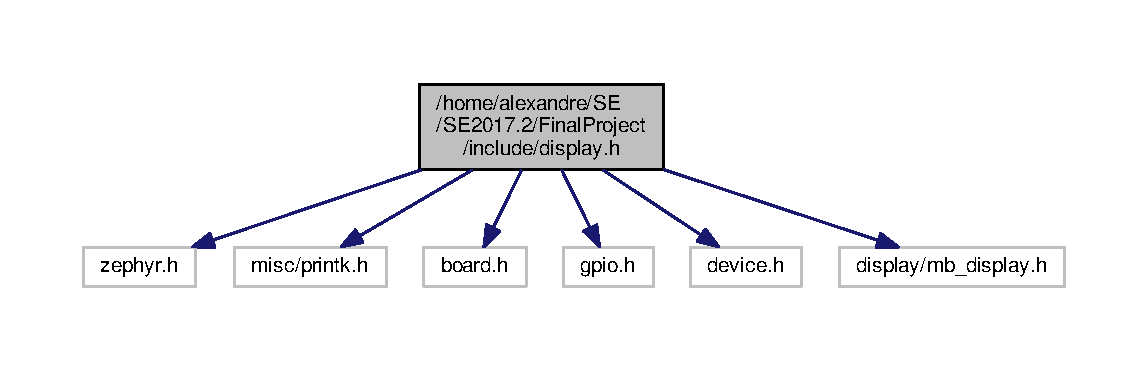
\includegraphics[width=350pt]{display_8h__incl}
\end{center}
\end{figure}
This graph shows which files directly or indirectly include this file\+:\nopagebreak
\begin{figure}[H]
\begin{center}
\leavevmode
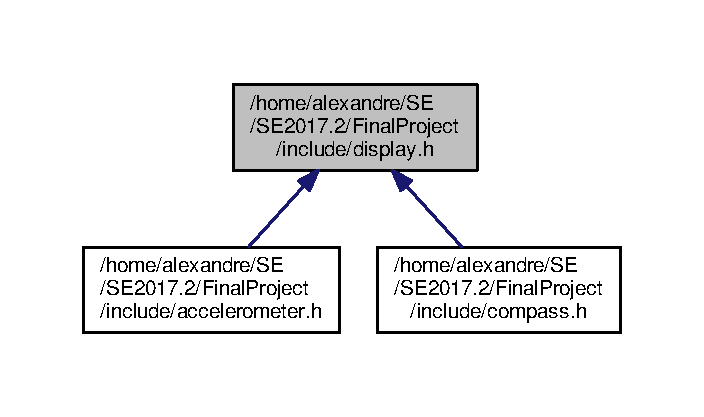
\includegraphics[width=338pt]{display_8h__dep__incl}
\end{center}
\end{figure}
\subsection*{Macros}
\begin{DoxyCompactItemize}
\item 
\#define \hyperlink{display_8h_ae0cf4db10c902d16029c235d0cf28ca6}{S\+C\+R\+E\+E\+N\+\_\+\+D\+U\+R\+A\+T\+I\+ON}~300
\end{DoxyCompactItemize}
\subsection*{Functions}
\begin{DoxyCompactItemize}
\item 
void \hyperlink{display_8h_ab0ca066858a1f39e7a56c4da7da98543}{print\+\_\+string\+\_\+to\+\_\+display} (const char $\ast$text, int ms\+\_\+duration)
\begin{DoxyCompactList}\small\item\em print\+\_\+string\+\_\+to\+\_\+display Scrolls text on the display \end{DoxyCompactList}\item 
void \hyperlink{display_8h_a0df8f7e68561180aeedcc85a138b2f89}{print\+\_\+int\+\_\+to\+\_\+display} (uint8\+\_\+t number, int ms\+\_\+duration)
\begin{DoxyCompactList}\small\item\em print\+\_\+int\+\_\+to\+\_\+display Scrolls a number on the screen \end{DoxyCompactList}\item 
void \hyperlink{display_8h_a431d770d374d4520da751dfafbce7059}{print\+\_\+double\+\_\+to\+\_\+display} (double number, int ms\+\_\+duration)
\begin{DoxyCompactList}\small\item\em print\+\_\+double\+\_\+to\+\_\+display Displays a floating-\/point number on the display \end{DoxyCompactList}\item 
void \hyperlink{display_8h_aad5f1cc6c2f47c2a58c7749181a756a6}{print\+\_\+image\+\_\+to\+\_\+display} (const struct mb\+\_\+image $\ast$img)
\begin{DoxyCompactList}\small\item\em print\+\_\+image\+\_\+to\+\_\+display Shows an image on the display for 1 second \end{DoxyCompactList}\item 
void \hyperlink{display_8h_ac1486c1dea925018d24334240a13261e}{clear\+\_\+display} ()
\begin{DoxyCompactList}\small\item\em clear\+\_\+display \end{DoxyCompactList}\end{DoxyCompactItemize}


\subsection{Macro Definition Documentation}
\index{display.\+h@{display.\+h}!S\+C\+R\+E\+E\+N\+\_\+\+D\+U\+R\+A\+T\+I\+ON@{S\+C\+R\+E\+E\+N\+\_\+\+D\+U\+R\+A\+T\+I\+ON}}
\index{S\+C\+R\+E\+E\+N\+\_\+\+D\+U\+R\+A\+T\+I\+ON@{S\+C\+R\+E\+E\+N\+\_\+\+D\+U\+R\+A\+T\+I\+ON}!display.\+h@{display.\+h}}
\subsubsection[{\texorpdfstring{S\+C\+R\+E\+E\+N\+\_\+\+D\+U\+R\+A\+T\+I\+ON}{SCREEN_DURATION}}]{\setlength{\rightskip}{0pt plus 5cm}\#define S\+C\+R\+E\+E\+N\+\_\+\+D\+U\+R\+A\+T\+I\+ON~300}\hypertarget{display_8h_ae0cf4db10c902d16029c235d0cf28ca6}{}\label{display_8h_ae0cf4db10c902d16029c235d0cf28ca6}


\subsection{Function Documentation}
\index{display.\+h@{display.\+h}!clear\+\_\+display@{clear\+\_\+display}}
\index{clear\+\_\+display@{clear\+\_\+display}!display.\+h@{display.\+h}}
\subsubsection[{\texorpdfstring{clear\+\_\+display()}{clear_display()}}]{\setlength{\rightskip}{0pt plus 5cm}void clear\+\_\+display (
\begin{DoxyParamCaption}
{}
\end{DoxyParamCaption}
)}\hypertarget{display_8h_ac1486c1dea925018d24334240a13261e}{}\label{display_8h_ac1486c1dea925018d24334240a13261e}


clear\+\_\+display 

Resets the display \index{display.\+h@{display.\+h}!print\+\_\+double\+\_\+to\+\_\+display@{print\+\_\+double\+\_\+to\+\_\+display}}
\index{print\+\_\+double\+\_\+to\+\_\+display@{print\+\_\+double\+\_\+to\+\_\+display}!display.\+h@{display.\+h}}
\subsubsection[{\texorpdfstring{print\+\_\+double\+\_\+to\+\_\+display(double number, int ms\+\_\+duration)}{print_double_to_display(double number, int ms_duration)}}]{\setlength{\rightskip}{0pt plus 5cm}void print\+\_\+double\+\_\+to\+\_\+display (
\begin{DoxyParamCaption}
\item[{double}]{number, }
\item[{int}]{ms\+\_\+duration}
\end{DoxyParamCaption}
)}\hypertarget{display_8h_a431d770d374d4520da751dfafbce7059}{}\label{display_8h_a431d770d374d4520da751dfafbce7059}


print\+\_\+double\+\_\+to\+\_\+display Displays a floating-\/point number on the display 


\begin{DoxyParams}{Parameters}
{\em number} & -\/ Double to be shown on display \\
\hline
{\em ms\+\_\+duration} & -\/ Duration of one character \\
\hline
\end{DoxyParams}
\index{display.\+h@{display.\+h}!print\+\_\+image\+\_\+to\+\_\+display@{print\+\_\+image\+\_\+to\+\_\+display}}
\index{print\+\_\+image\+\_\+to\+\_\+display@{print\+\_\+image\+\_\+to\+\_\+display}!display.\+h@{display.\+h}}
\subsubsection[{\texorpdfstring{print\+\_\+image\+\_\+to\+\_\+display(const struct mb\+\_\+image $\ast$img)}{print_image_to_display(const struct mb_image *img)}}]{\setlength{\rightskip}{0pt plus 5cm}void print\+\_\+image\+\_\+to\+\_\+display (
\begin{DoxyParamCaption}
\item[{const struct mb\+\_\+image $\ast$}]{img}
\end{DoxyParamCaption}
)}\hypertarget{display_8h_aad5f1cc6c2f47c2a58c7749181a756a6}{}\label{display_8h_aad5f1cc6c2f47c2a58c7749181a756a6}


print\+\_\+image\+\_\+to\+\_\+display Shows an image on the display for 1 second 


\begin{DoxyParams}{Parameters}
{\em img} & -\/ Image to be displayed \\
\hline
\end{DoxyParams}
\index{display.\+h@{display.\+h}!print\+\_\+int\+\_\+to\+\_\+display@{print\+\_\+int\+\_\+to\+\_\+display}}
\index{print\+\_\+int\+\_\+to\+\_\+display@{print\+\_\+int\+\_\+to\+\_\+display}!display.\+h@{display.\+h}}
\subsubsection[{\texorpdfstring{print\+\_\+int\+\_\+to\+\_\+display(uint8\+\_\+t number, int ms\+\_\+duration)}{print_int_to_display(uint8_t number, int ms_duration)}}]{\setlength{\rightskip}{0pt plus 5cm}void print\+\_\+int\+\_\+to\+\_\+display (
\begin{DoxyParamCaption}
\item[{uint8\+\_\+t}]{number, }
\item[{int}]{ms\+\_\+duration}
\end{DoxyParamCaption}
)}\hypertarget{display_8h_a0df8f7e68561180aeedcc85a138b2f89}{}\label{display_8h_a0df8f7e68561180aeedcc85a138b2f89}


print\+\_\+int\+\_\+to\+\_\+display Scrolls a number on the screen 


\begin{DoxyParams}{Parameters}
{\em number} & Integer to be shown on the display \\
\hline
{\em ms\+\_\+duration} & -\/ Duration of one character \\
\hline
\end{DoxyParams}
\index{display.\+h@{display.\+h}!print\+\_\+string\+\_\+to\+\_\+display@{print\+\_\+string\+\_\+to\+\_\+display}}
\index{print\+\_\+string\+\_\+to\+\_\+display@{print\+\_\+string\+\_\+to\+\_\+display}!display.\+h@{display.\+h}}
\subsubsection[{\texorpdfstring{print\+\_\+string\+\_\+to\+\_\+display(const char $\ast$text, int ms\+\_\+duration)}{print_string_to_display(const char *text, int ms_duration)}}]{\setlength{\rightskip}{0pt plus 5cm}void print\+\_\+string\+\_\+to\+\_\+display (
\begin{DoxyParamCaption}
\item[{const char $\ast$}]{text, }
\item[{int}]{ms\+\_\+duration}
\end{DoxyParamCaption}
)}\hypertarget{display_8h_ab0ca066858a1f39e7a56c4da7da98543}{}\label{display_8h_ab0ca066858a1f39e7a56c4da7da98543}


print\+\_\+string\+\_\+to\+\_\+display Scrolls text on the display 


\begin{DoxyParams}{Parameters}
{\em text} & -\/ Text to be shown \\
\hline
{\em ms\+\_\+duration} & -\/ Duration of one character \\
\hline
\end{DoxyParams}

\hypertarget{i2c__device_8h}{}\section{/home/alexandre/\+S\+E/\+S\+E2017.2/\+Final\+Project/include/i2c\+\_\+device.h File Reference}
\label{i2c__device_8h}\index{/home/alexandre/\+S\+E/\+S\+E2017.\+2/\+Final\+Project/include/i2c\+\_\+device.\+h@{/home/alexandre/\+S\+E/\+S\+E2017.\+2/\+Final\+Project/include/i2c\+\_\+device.\+h}}
{\ttfamily \#include \char`\"{}version.\+h\char`\"{}}\\*
{\ttfamily \#include \char`\"{}i2c\+\_\+util.\+h\char`\"{}}\\*
{\ttfamily \#include $<$stdint.\+h$>$}\\*
Include dependency graph for i2c\+\_\+device.\+h\+:\nopagebreak
\begin{figure}[H]
\begin{center}
\leavevmode
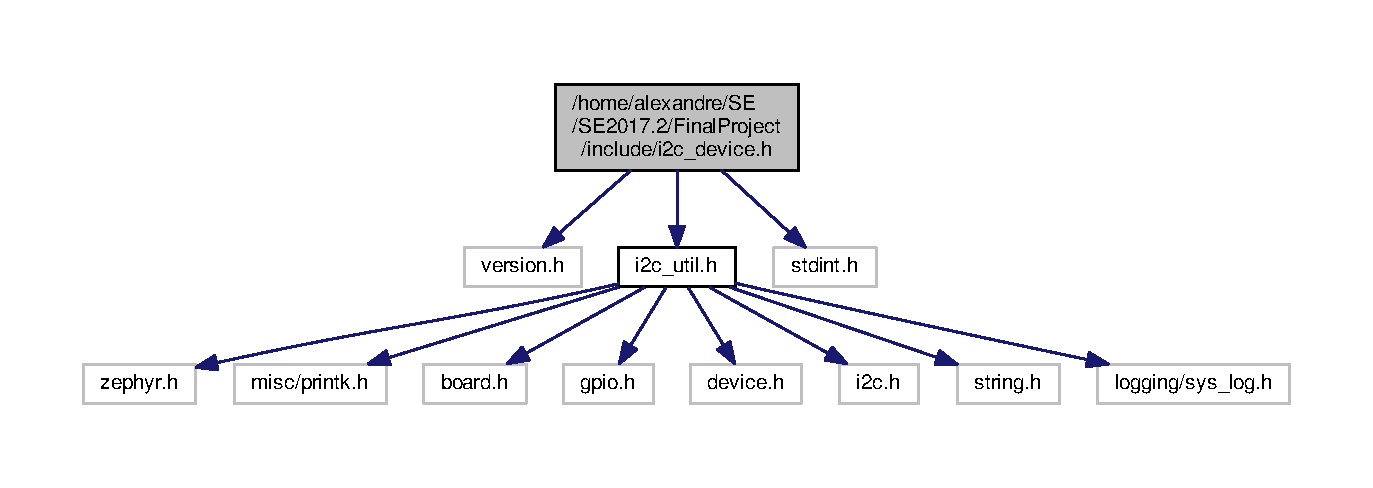
\includegraphics[width=350pt]{i2c__device_8h__incl}
\end{center}
\end{figure}
This graph shows which files directly or indirectly include this file\+:\nopagebreak
\begin{figure}[H]
\begin{center}
\leavevmode
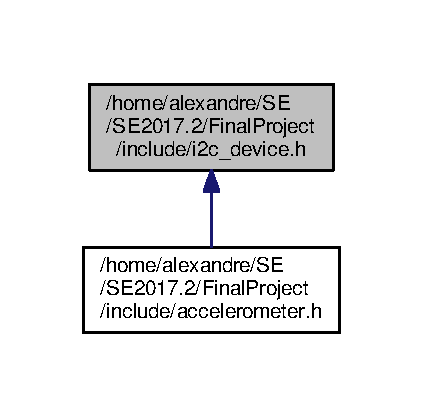
\includegraphics[width=203pt]{i2c__device_8h__dep__incl}
\end{center}
\end{figure}
\subsection*{Functions}
\begin{DoxyCompactItemize}
\item 
void \hyperlink{i2c__device_8h_a4987d8d30a75237baf8a7a13c03dffe8}{accelerometer\+\_\+init} (void)
\begin{DoxyCompactList}\small\item\em accelerometer\+\_\+init \end{DoxyCompactList}\item 
void \hyperlink{i2c__device_8h_a9974dbc346f9bc063734b1024ef38186}{accelerometer\+\_\+standby} (void)
\begin{DoxyCompactList}\small\item\em accelerometer\+\_\+standby \end{DoxyCompactList}\item 
void \hyperlink{i2c__device_8h_ad2c3341a2e62d06966c10af71d4cc2ba}{accelerometer\+\_\+active} (void)
\begin{DoxyCompactList}\small\item\em accelerometer\+\_\+active Change accelerometer device status to active \end{DoxyCompactList}\item 
void \hyperlink{i2c__device_8h_a6b00d3dd6886413e8360d7f823dfd917}{read\+\_\+from\+\_\+accelerometer} (uint8\+\_\+t $\ast$data)
\begin{DoxyCompactList}\small\item\em read\+\_\+from\+\_\+accelerometer Read the raw x, y and z values from the accelerometer device \end{DoxyCompactList}\item 
void \hyperlink{i2c__device_8h_a8dec46d68222e3753f9e896cb89f2eff}{compass\+\_\+init} (void)
\begin{DoxyCompactList}\small\item\em compass\+\_\+init \end{DoxyCompactList}\item 
void \hyperlink{i2c__device_8h_aedae8d7581a0a5c331739312b99501b6}{compass\+\_\+active} (void)
\begin{DoxyCompactList}\small\item\em compass\+\_\+active \end{DoxyCompactList}\item 
void \hyperlink{i2c__device_8h_affcdec32838de9a8c68ab57563800c3b}{compass\+\_\+standby} (void)
\begin{DoxyCompactList}\small\item\em compass\+\_\+standby \end{DoxyCompactList}\item 
void \hyperlink{i2c__device_8h_ad868676abc1544ced1e717918d810070}{read\+\_\+from\+\_\+compass} (uint8\+\_\+t $\ast$data)
\begin{DoxyCompactList}\small\item\em read\+\_\+from\+\_\+compass Read the raw x, y and z values from the magnetometer device \end{DoxyCompactList}\end{DoxyCompactItemize}


\subsection{Function Documentation}
\index{i2c\+\_\+device.\+h@{i2c\+\_\+device.\+h}!accelerometer\+\_\+active@{accelerometer\+\_\+active}}
\index{accelerometer\+\_\+active@{accelerometer\+\_\+active}!i2c\+\_\+device.\+h@{i2c\+\_\+device.\+h}}
\subsubsection[{\texorpdfstring{accelerometer\+\_\+active(void)}{accelerometer_active(void)}}]{\setlength{\rightskip}{0pt plus 5cm}void accelerometer\+\_\+active (
\begin{DoxyParamCaption}
\item[{void}]{}
\end{DoxyParamCaption}
)}\hypertarget{i2c__device_8h_ad2c3341a2e62d06966c10af71d4cc2ba}{}\label{i2c__device_8h_ad2c3341a2e62d06966c10af71d4cc2ba}


accelerometer\+\_\+active Change accelerometer device status to active 

\index{i2c\+\_\+device.\+h@{i2c\+\_\+device.\+h}!accelerometer\+\_\+init@{accelerometer\+\_\+init}}
\index{accelerometer\+\_\+init@{accelerometer\+\_\+init}!i2c\+\_\+device.\+h@{i2c\+\_\+device.\+h}}
\subsubsection[{\texorpdfstring{accelerometer\+\_\+init(void)}{accelerometer_init(void)}}]{\setlength{\rightskip}{0pt plus 5cm}void accelerometer\+\_\+init (
\begin{DoxyParamCaption}
\item[{void}]{}
\end{DoxyParamCaption}
)}\hypertarget{i2c__device_8h_a4987d8d30a75237baf8a7a13c03dffe8}{}\label{i2c__device_8h_a4987d8d30a75237baf8a7a13c03dffe8}


accelerometer\+\_\+init 

Configure the accelerometer device for use \index{i2c\+\_\+device.\+h@{i2c\+\_\+device.\+h}!accelerometer\+\_\+standby@{accelerometer\+\_\+standby}}
\index{accelerometer\+\_\+standby@{accelerometer\+\_\+standby}!i2c\+\_\+device.\+h@{i2c\+\_\+device.\+h}}
\subsubsection[{\texorpdfstring{accelerometer\+\_\+standby(void)}{accelerometer_standby(void)}}]{\setlength{\rightskip}{0pt plus 5cm}void accelerometer\+\_\+standby (
\begin{DoxyParamCaption}
\item[{void}]{}
\end{DoxyParamCaption}
)}\hypertarget{i2c__device_8h_a9974dbc346f9bc063734b1024ef38186}{}\label{i2c__device_8h_a9974dbc346f9bc063734b1024ef38186}


accelerometer\+\_\+standby 

Change accelerometer device status to \char`\"{}standby\char`\"{} \index{i2c\+\_\+device.\+h@{i2c\+\_\+device.\+h}!compass\+\_\+active@{compass\+\_\+active}}
\index{compass\+\_\+active@{compass\+\_\+active}!i2c\+\_\+device.\+h@{i2c\+\_\+device.\+h}}
\subsubsection[{\texorpdfstring{compass\+\_\+active(void)}{compass_active(void)}}]{\setlength{\rightskip}{0pt plus 5cm}void compass\+\_\+active (
\begin{DoxyParamCaption}
\item[{void}]{}
\end{DoxyParamCaption}
)}\hypertarget{i2c__device_8h_aedae8d7581a0a5c331739312b99501b6}{}\label{i2c__device_8h_aedae8d7581a0a5c331739312b99501b6}


compass\+\_\+active 

Change magnometer device status to \char`\"{}active\char`\"{} \index{i2c\+\_\+device.\+h@{i2c\+\_\+device.\+h}!compass\+\_\+init@{compass\+\_\+init}}
\index{compass\+\_\+init@{compass\+\_\+init}!i2c\+\_\+device.\+h@{i2c\+\_\+device.\+h}}
\subsubsection[{\texorpdfstring{compass\+\_\+init(void)}{compass_init(void)}}]{\setlength{\rightskip}{0pt plus 5cm}void compass\+\_\+init (
\begin{DoxyParamCaption}
\item[{void}]{}
\end{DoxyParamCaption}
)}\hypertarget{i2c__device_8h_a8dec46d68222e3753f9e896cb89f2eff}{}\label{i2c__device_8h_a8dec46d68222e3753f9e896cb89f2eff}


compass\+\_\+init 

Configure the magnetometer device for use \index{i2c\+\_\+device.\+h@{i2c\+\_\+device.\+h}!compass\+\_\+standby@{compass\+\_\+standby}}
\index{compass\+\_\+standby@{compass\+\_\+standby}!i2c\+\_\+device.\+h@{i2c\+\_\+device.\+h}}
\subsubsection[{\texorpdfstring{compass\+\_\+standby(void)}{compass_standby(void)}}]{\setlength{\rightskip}{0pt plus 5cm}void compass\+\_\+standby (
\begin{DoxyParamCaption}
\item[{void}]{}
\end{DoxyParamCaption}
)}\hypertarget{i2c__device_8h_affcdec32838de9a8c68ab57563800c3b}{}\label{i2c__device_8h_affcdec32838de9a8c68ab57563800c3b}


compass\+\_\+standby 

Change magnetometer device status to \char`\"{}standby\char`\"{} \index{i2c\+\_\+device.\+h@{i2c\+\_\+device.\+h}!read\+\_\+from\+\_\+accelerometer@{read\+\_\+from\+\_\+accelerometer}}
\index{read\+\_\+from\+\_\+accelerometer@{read\+\_\+from\+\_\+accelerometer}!i2c\+\_\+device.\+h@{i2c\+\_\+device.\+h}}
\subsubsection[{\texorpdfstring{read\+\_\+from\+\_\+accelerometer(uint8\+\_\+t $\ast$data)}{read_from_accelerometer(uint8_t *data)}}]{\setlength{\rightskip}{0pt plus 5cm}void read\+\_\+from\+\_\+accelerometer (
\begin{DoxyParamCaption}
\item[{uint8\+\_\+t $\ast$}]{data}
\end{DoxyParamCaption}
)}\hypertarget{i2c__device_8h_a6b00d3dd6886413e8360d7f823dfd917}{}\label{i2c__device_8h_a6b00d3dd6886413e8360d7f823dfd917}


read\+\_\+from\+\_\+accelerometer Read the raw x, y and z values from the accelerometer device 


\begin{DoxyParams}{Parameters}
{\em dst} & -\/ destination of the x, y, z data. \\
\hline
\end{DoxyParams}
\index{i2c\+\_\+device.\+h@{i2c\+\_\+device.\+h}!read\+\_\+from\+\_\+compass@{read\+\_\+from\+\_\+compass}}
\index{read\+\_\+from\+\_\+compass@{read\+\_\+from\+\_\+compass}!i2c\+\_\+device.\+h@{i2c\+\_\+device.\+h}}
\subsubsection[{\texorpdfstring{read\+\_\+from\+\_\+compass(uint8\+\_\+t $\ast$data)}{read_from_compass(uint8_t *data)}}]{\setlength{\rightskip}{0pt plus 5cm}void read\+\_\+from\+\_\+compass (
\begin{DoxyParamCaption}
\item[{uint8\+\_\+t $\ast$}]{data}
\end{DoxyParamCaption}
)}\hypertarget{i2c__device_8h_ad868676abc1544ced1e717918d810070}{}\label{i2c__device_8h_ad868676abc1544ced1e717918d810070}


read\+\_\+from\+\_\+compass Read the raw x, y and z values from the magnetometer device 


\begin{DoxyParams}{Parameters}
{\em data} & -\/ destination for the raw x, y, z data. \\
\hline
\end{DoxyParams}

\hypertarget{i2c__util_8h}{}\section{/home/alexandre/\+S\+E/\+S\+E2017.2/\+Final\+Project/include/i2c\+\_\+util.h File Reference}
\label{i2c__util_8h}\index{/home/alexandre/\+S\+E/\+S\+E2017.\+2/\+Final\+Project/include/i2c\+\_\+util.\+h@{/home/alexandre/\+S\+E/\+S\+E2017.\+2/\+Final\+Project/include/i2c\+\_\+util.\+h}}
{\ttfamily \#include $<$zephyr.\+h$>$}\\*
{\ttfamily \#include $<$misc/printk.\+h$>$}\\*
{\ttfamily \#include $<$board.\+h$>$}\\*
{\ttfamily \#include $<$gpio.\+h$>$}\\*
{\ttfamily \#include $<$device.\+h$>$}\\*
{\ttfamily \#include $<$i2c.\+h$>$}\\*
{\ttfamily \#include $<$string.\+h$>$}\\*
{\ttfamily \#include $<$logging/sys\+\_\+log.\+h$>$}\\*
Include dependency graph for i2c\+\_\+util.\+h\+:\nopagebreak
\begin{figure}[H]
\begin{center}
\leavevmode
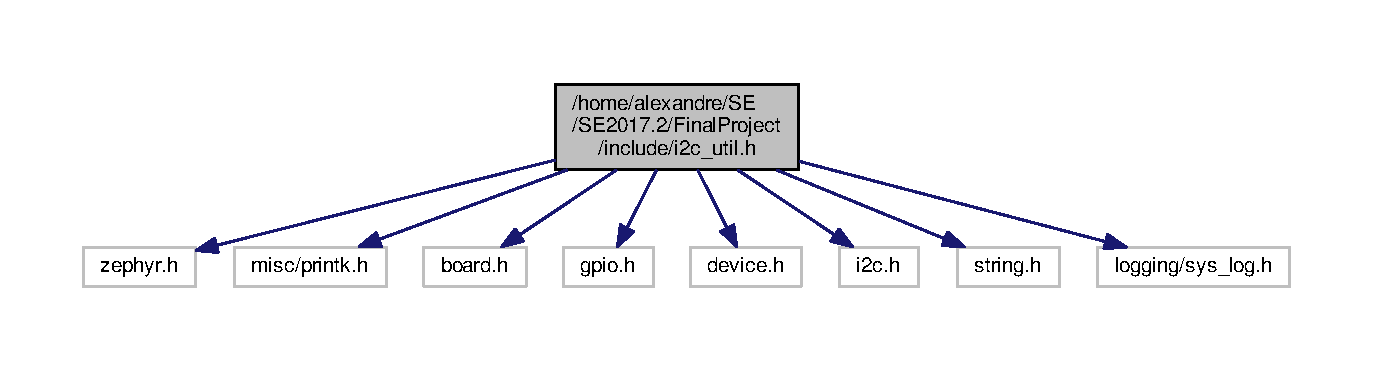
\includegraphics[width=350pt]{i2c__util_8h__incl}
\end{center}
\end{figure}
This graph shows which files directly or indirectly include this file\+:\nopagebreak
\begin{figure}[H]
\begin{center}
\leavevmode
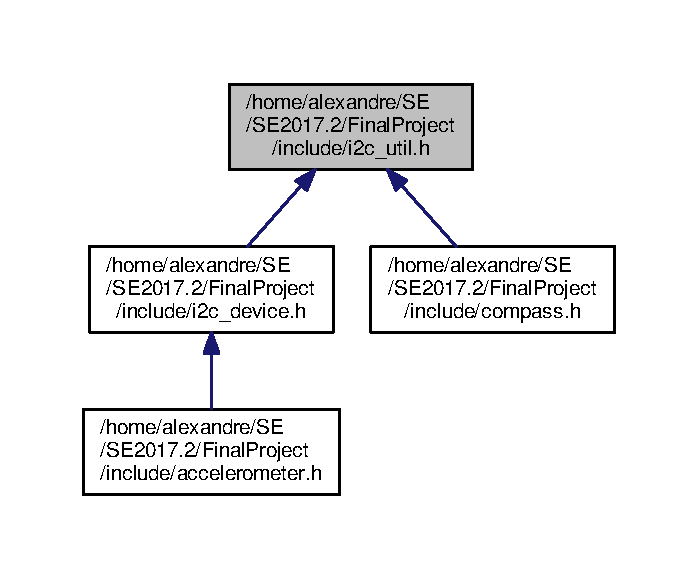
\includegraphics[width=335pt]{i2c__util_8h__dep__incl}
\end{center}
\end{figure}
\subsection*{Classes}
\begin{DoxyCompactItemize}
\item 
struct \hyperlink{structi2c__dev}{i2c\+\_\+dev}
\end{DoxyCompactItemize}
\subsection*{Macros}
\begin{DoxyCompactItemize}
\item 
\#define \hyperlink{i2c__util_8h_ac5b2cb2d6ae6b5526953a00f765a23e4}{S\+Y\+S\+\_\+\+L\+O\+G\+\_\+\+D\+O\+M\+A\+IN}~\char`\"{}P\+R\+O\+J\+E\+CT\char`\"{}
\item 
\#define \hyperlink{i2c__util_8h_a48e1e64a2a8c3e1e1df44760d2a73eaa}{I2\+C\+\_\+\+D\+E\+V\+I\+C\+E\+\_\+\+N\+A\+M\+E\+\_\+\+L\+E\+N\+G\+TH}~10
\end{DoxyCompactItemize}
\subsection*{Functions}
\begin{DoxyCompactItemize}
\item 
int \hyperlink{i2c__util_8h_a94dc84189a2c77ce509621dc4adb8150}{i2c\+\_\+util\+\_\+dev\+\_\+init} (struct \hyperlink{structi2c__dev}{i2c\+\_\+dev} $\ast$\hyperlink{structi2c__dev}{i2c\+\_\+dev}, u16\+\_\+t addr, const char $\ast$name, u8\+\_\+t reg\+\_\+test, u8\+\_\+t reg\+\_\+test\+\_\+expected\+\_\+val)
\item 
int \hyperlink{i2c__util_8h_a9bdf91cfea8b14d68bc7d8819e7ba742}{i2c\+\_\+util\+\_\+write\+\_\+bytes} (struct \hyperlink{structi2c__dev}{i2c\+\_\+dev} $\ast$\hyperlink{structi2c__dev}{i2c\+\_\+dev}, u8\+\_\+t reg, u8\+\_\+t $\ast$data, u32\+\_\+t num\+\_\+bytes)
\item 
int \hyperlink{i2c__util_8h_a7510a339f80427d63e309fd8b6613ce7}{i2c\+\_\+util\+\_\+read\+\_\+bytes} (struct \hyperlink{structi2c__dev}{i2c\+\_\+dev} $\ast$\hyperlink{structi2c__dev}{i2c\+\_\+dev}, u8\+\_\+t reg, u8\+\_\+t $\ast$data, u32\+\_\+t num\+\_\+bytes)
\item 
int \hyperlink{i2c__util_8h_a7879cbd3e3c4f64e2b36ef77aaf0ec85}{i2c\+\_\+util\+\_\+test\+\_\+connection} (struct \hyperlink{structi2c__dev}{i2c\+\_\+dev} $\ast$\hyperlink{structi2c__dev}{i2c\+\_\+dev})
\end{DoxyCompactItemize}


\subsection{Macro Definition Documentation}
\index{i2c\+\_\+util.\+h@{i2c\+\_\+util.\+h}!I2\+C\+\_\+\+D\+E\+V\+I\+C\+E\+\_\+\+N\+A\+M\+E\+\_\+\+L\+E\+N\+G\+TH@{I2\+C\+\_\+\+D\+E\+V\+I\+C\+E\+\_\+\+N\+A\+M\+E\+\_\+\+L\+E\+N\+G\+TH}}
\index{I2\+C\+\_\+\+D\+E\+V\+I\+C\+E\+\_\+\+N\+A\+M\+E\+\_\+\+L\+E\+N\+G\+TH@{I2\+C\+\_\+\+D\+E\+V\+I\+C\+E\+\_\+\+N\+A\+M\+E\+\_\+\+L\+E\+N\+G\+TH}!i2c\+\_\+util.\+h@{i2c\+\_\+util.\+h}}
\subsubsection[{\texorpdfstring{I2\+C\+\_\+\+D\+E\+V\+I\+C\+E\+\_\+\+N\+A\+M\+E\+\_\+\+L\+E\+N\+G\+TH}{I2C_DEVICE_NAME_LENGTH}}]{\setlength{\rightskip}{0pt plus 5cm}\#define I2\+C\+\_\+\+D\+E\+V\+I\+C\+E\+\_\+\+N\+A\+M\+E\+\_\+\+L\+E\+N\+G\+TH~10}\hypertarget{i2c__util_8h_a48e1e64a2a8c3e1e1df44760d2a73eaa}{}\label{i2c__util_8h_a48e1e64a2a8c3e1e1df44760d2a73eaa}
\index{i2c\+\_\+util.\+h@{i2c\+\_\+util.\+h}!S\+Y\+S\+\_\+\+L\+O\+G\+\_\+\+D\+O\+M\+A\+IN@{S\+Y\+S\+\_\+\+L\+O\+G\+\_\+\+D\+O\+M\+A\+IN}}
\index{S\+Y\+S\+\_\+\+L\+O\+G\+\_\+\+D\+O\+M\+A\+IN@{S\+Y\+S\+\_\+\+L\+O\+G\+\_\+\+D\+O\+M\+A\+IN}!i2c\+\_\+util.\+h@{i2c\+\_\+util.\+h}}
\subsubsection[{\texorpdfstring{S\+Y\+S\+\_\+\+L\+O\+G\+\_\+\+D\+O\+M\+A\+IN}{SYS_LOG_DOMAIN}}]{\setlength{\rightskip}{0pt plus 5cm}\#define S\+Y\+S\+\_\+\+L\+O\+G\+\_\+\+D\+O\+M\+A\+IN~\char`\"{}P\+R\+O\+J\+E\+CT\char`\"{}}\hypertarget{i2c__util_8h_ac5b2cb2d6ae6b5526953a00f765a23e4}{}\label{i2c__util_8h_ac5b2cb2d6ae6b5526953a00f765a23e4}


\subsection{Function Documentation}
\index{i2c\+\_\+util.\+h@{i2c\+\_\+util.\+h}!i2c\+\_\+util\+\_\+dev\+\_\+init@{i2c\+\_\+util\+\_\+dev\+\_\+init}}
\index{i2c\+\_\+util\+\_\+dev\+\_\+init@{i2c\+\_\+util\+\_\+dev\+\_\+init}!i2c\+\_\+util.\+h@{i2c\+\_\+util.\+h}}
\subsubsection[{\texorpdfstring{i2c\+\_\+util\+\_\+dev\+\_\+init(struct i2c\+\_\+dev $\ast$i2c\+\_\+dev, u16\+\_\+t addr, const char $\ast$name, u8\+\_\+t reg\+\_\+test, u8\+\_\+t reg\+\_\+test\+\_\+expected\+\_\+val)}{i2c_util_dev_init(struct i2c_dev *i2c_dev, u16_t addr, const char *name, u8_t reg_test, u8_t reg_test_expected_val)}}]{\setlength{\rightskip}{0pt plus 5cm}int i2c\+\_\+util\+\_\+dev\+\_\+init (
\begin{DoxyParamCaption}
\item[{struct {\bf i2c\+\_\+dev} $\ast$}]{i2c\+\_\+dev, }
\item[{u16\+\_\+t}]{addr, }
\item[{const char $\ast$}]{name, }
\item[{u8\+\_\+t}]{reg\+\_\+test, }
\item[{u8\+\_\+t}]{reg\+\_\+test\+\_\+expected\+\_\+val}
\end{DoxyParamCaption}
)}\hypertarget{i2c__util_8h_a94dc84189a2c77ce509621dc4adb8150}{}\label{i2c__util_8h_a94dc84189a2c77ce509621dc4adb8150}
\index{i2c\+\_\+util.\+h@{i2c\+\_\+util.\+h}!i2c\+\_\+util\+\_\+read\+\_\+bytes@{i2c\+\_\+util\+\_\+read\+\_\+bytes}}
\index{i2c\+\_\+util\+\_\+read\+\_\+bytes@{i2c\+\_\+util\+\_\+read\+\_\+bytes}!i2c\+\_\+util.\+h@{i2c\+\_\+util.\+h}}
\subsubsection[{\texorpdfstring{i2c\+\_\+util\+\_\+read\+\_\+bytes(struct i2c\+\_\+dev $\ast$i2c\+\_\+dev, u8\+\_\+t reg, u8\+\_\+t $\ast$data, u32\+\_\+t num\+\_\+bytes)}{i2c_util_read_bytes(struct i2c_dev *i2c_dev, u8_t reg, u8_t *data, u32_t num_bytes)}}]{\setlength{\rightskip}{0pt plus 5cm}int i2c\+\_\+util\+\_\+read\+\_\+bytes (
\begin{DoxyParamCaption}
\item[{struct {\bf i2c\+\_\+dev} $\ast$}]{i2c\+\_\+dev, }
\item[{u8\+\_\+t}]{reg, }
\item[{u8\+\_\+t $\ast$}]{data, }
\item[{u32\+\_\+t}]{num\+\_\+bytes}
\end{DoxyParamCaption}
)}\hypertarget{i2c__util_8h_a7510a339f80427d63e309fd8b6613ce7}{}\label{i2c__util_8h_a7510a339f80427d63e309fd8b6613ce7}
\index{i2c\+\_\+util.\+h@{i2c\+\_\+util.\+h}!i2c\+\_\+util\+\_\+test\+\_\+connection@{i2c\+\_\+util\+\_\+test\+\_\+connection}}
\index{i2c\+\_\+util\+\_\+test\+\_\+connection@{i2c\+\_\+util\+\_\+test\+\_\+connection}!i2c\+\_\+util.\+h@{i2c\+\_\+util.\+h}}
\subsubsection[{\texorpdfstring{i2c\+\_\+util\+\_\+test\+\_\+connection(struct i2c\+\_\+dev $\ast$i2c\+\_\+dev)}{i2c_util_test_connection(struct i2c_dev *i2c_dev)}}]{\setlength{\rightskip}{0pt plus 5cm}int i2c\+\_\+util\+\_\+test\+\_\+connection (
\begin{DoxyParamCaption}
\item[{struct {\bf i2c\+\_\+dev} $\ast$}]{i2c\+\_\+dev}
\end{DoxyParamCaption}
)}\hypertarget{i2c__util_8h_a7879cbd3e3c4f64e2b36ef77aaf0ec85}{}\label{i2c__util_8h_a7879cbd3e3c4f64e2b36ef77aaf0ec85}
\index{i2c\+\_\+util.\+h@{i2c\+\_\+util.\+h}!i2c\+\_\+util\+\_\+write\+\_\+bytes@{i2c\+\_\+util\+\_\+write\+\_\+bytes}}
\index{i2c\+\_\+util\+\_\+write\+\_\+bytes@{i2c\+\_\+util\+\_\+write\+\_\+bytes}!i2c\+\_\+util.\+h@{i2c\+\_\+util.\+h}}
\subsubsection[{\texorpdfstring{i2c\+\_\+util\+\_\+write\+\_\+bytes(struct i2c\+\_\+dev $\ast$i2c\+\_\+dev, u8\+\_\+t reg, u8\+\_\+t $\ast$data, u32\+\_\+t num\+\_\+bytes)}{i2c_util_write_bytes(struct i2c_dev *i2c_dev, u8_t reg, u8_t *data, u32_t num_bytes)}}]{\setlength{\rightskip}{0pt plus 5cm}int i2c\+\_\+util\+\_\+write\+\_\+bytes (
\begin{DoxyParamCaption}
\item[{struct {\bf i2c\+\_\+dev} $\ast$}]{i2c\+\_\+dev, }
\item[{u8\+\_\+t}]{reg, }
\item[{u8\+\_\+t $\ast$}]{data, }
\item[{u32\+\_\+t}]{num\+\_\+bytes}
\end{DoxyParamCaption}
)}\hypertarget{i2c__util_8h_a9bdf91cfea8b14d68bc7d8819e7ba742}{}\label{i2c__util_8h_a9bdf91cfea8b14d68bc7d8819e7ba742}

\hypertarget{state__machine_8h}{}\section{/home/alexandre/\+S\+E/\+S\+E2017.2/\+Final\+Project/include/state\+\_\+machine.h File Reference}
\label{state__machine_8h}\index{/home/alexandre/\+S\+E/\+S\+E2017.\+2/\+Final\+Project/include/state\+\_\+machine.\+h@{/home/alexandre/\+S\+E/\+S\+E2017.\+2/\+Final\+Project/include/state\+\_\+machine.\+h}}
\subsection*{Classes}
\begin{DoxyCompactItemize}
\item 
struct \hyperlink{structstate__machine__t}{state\+\_\+machine\+\_\+t}
\end{DoxyCompactItemize}
\subsection*{Typedefs}
\begin{DoxyCompactItemize}
\item 
typedef enum  \{ ... \}  \hyperlink{state__machine_8h_aa7e27c2c7466e74443d5b84380bdd4c0}{state\+\_\+t}
\begin{DoxyCompactList}\small\item\em state\+\_\+t Enum of possible device states /$\ast$$\ast$ \end{DoxyCompactList}\item 
typedef enum  \{ ... \}  \hyperlink{state__machine_8h_ae25a04191e5c569bf374e7a804228d49}{event\+\_\+t}
\begin{DoxyCompactList}\small\item\em event\+\_\+t Enum of triggerable events \end{DoxyCompactList}\end{DoxyCompactItemize}
\subsection*{Enumerations}
\begin{DoxyCompactItemize}
\item 
enum \{ \\*
\hyperlink{state__machine_8h_a99fb83031ce9923c84392b4e92f956b5a5c1177d066ef87bb2901278d1d1f76f8}{T\+E\+X\+T\+\_\+\+D\+I\+S\+P\+L\+AY}, 
\hyperlink{state__machine_8h_a99fb83031ce9923c84392b4e92f956b5a227f5dfe4607bb6c220798f2f318f73d}{A\+C\+C\+E\+L\+E\+R\+O\+M\+E\+T\+ER}, 
\hyperlink{state__machine_8h_a99fb83031ce9923c84392b4e92f956b5a3816a21235046441a516c9435b144aee}{C\+O\+M\+P\+A\+SS}, 
\hyperlink{state__machine_8h_a99fb83031ce9923c84392b4e92f956b5ad29db38aeccaf1d78edb295a0f402fe1}{T\+H\+E\+R\+M\+O\+M\+E\+T\+ER}, 
\\*
\hyperlink{state__machine_8h_a99fb83031ce9923c84392b4e92f956b5acf9d75f7b1a34d02c9d810281f51cf2a}{B\+L\+U\+E\+T\+O\+O\+TH}
 \}\begin{DoxyCompactList}\small\item\em state\+\_\+t Enum of possible device states /$\ast$$\ast$ \end{DoxyCompactList}
\item 
enum \{ \hyperlink{state__machine_8h_abc6126af1d45847bc59afa0aa3216b04a0d56a81c8a754989f46db0d1ca6ca16e}{B\+U\+T\+T\+O\+N\+\_\+A}, 
\hyperlink{state__machine_8h_abc6126af1d45847bc59afa0aa3216b04a8ffa84a83c0c23197c288f9c492dac40}{B\+U\+T\+T\+O\+N\+\_\+B}
 \}\begin{DoxyCompactList}\small\item\em event\+\_\+t Enum of triggerable events \end{DoxyCompactList}
\end{DoxyCompactItemize}
\subsection*{Functions}
\begin{DoxyCompactItemize}
\item 
void \hyperlink{state__machine_8h_af0500e1eccc31b02cf60d7402e346cd2}{state\+\_\+machine\+\_\+change\+\_\+state} (\hyperlink{state__machine_8h_ae25a04191e5c569bf374e7a804228d49}{event\+\_\+t} event)
\begin{DoxyCompactList}\small\item\em scroll\+\_\+\+Text Shows \char`\"{}\+E\+C\+O\+M042.\+2017.\+2\char`\"{} scrolling in the display \end{DoxyCompactList}\item 
void \hyperlink{state__machine_8h_a6c15ed9ec59e864ffee5d50c5f1b9118}{scroll\+\_\+\+Text} (void)
\item 
static void \hyperlink{state__machine_8h_a6e254a25748734edf2fcc84d12d4f390}{bluetooth} (void)
\item 
void \hyperlink{state__machine_8h_a5fd9d0df63f9fc4e4f9392fcaa45f67b}{show\+\_\+temperature} (void)
\begin{DoxyCompactList}\small\item\em Shows current temperature in Celsius on the display. \end{DoxyCompactList}\item 
\hyperlink{structstate__machine__t}{state\+\_\+machine\+\_\+t} $\ast$ \hyperlink{state__machine_8h_a18d8983c509c9a95a33331ba2b2bafc3}{get\+\_\+current\+\_\+state} (void)
\begin{DoxyCompactList}\small\item\em get\+\_\+current\+\_\+state Get the current machine state from the state machine \end{DoxyCompactList}\end{DoxyCompactItemize}


\subsection{Typedef Documentation}
\index{state\+\_\+machine.\+h@{state\+\_\+machine.\+h}!event\+\_\+t@{event\+\_\+t}}
\index{event\+\_\+t@{event\+\_\+t}!state\+\_\+machine.\+h@{state\+\_\+machine.\+h}}
\subsubsection[{\texorpdfstring{event\+\_\+t}{event_t}}]{\setlength{\rightskip}{0pt plus 5cm}typedef \{ ... \}   {\bf event\+\_\+t}}\hypertarget{state__machine_8h_ae25a04191e5c569bf374e7a804228d49}{}\label{state__machine_8h_ae25a04191e5c569bf374e7a804228d49}


event\+\_\+t Enum of triggerable events 

/$\ast$$\ast$ $\ast$/$\ast$$\ast$ \index{state\+\_\+machine.\+h@{state\+\_\+machine.\+h}!state\+\_\+t@{state\+\_\+t}}
\index{state\+\_\+t@{state\+\_\+t}!state\+\_\+machine.\+h@{state\+\_\+machine.\+h}}
\subsubsection[{\texorpdfstring{state\+\_\+t}{state_t}}]{\setlength{\rightskip}{0pt plus 5cm}typedef \{ ... \}   {\bf state\+\_\+t}}\hypertarget{state__machine_8h_aa7e27c2c7466e74443d5b84380bdd4c0}{}\label{state__machine_8h_aa7e27c2c7466e74443d5b84380bdd4c0}


state\+\_\+t Enum of possible device states /$\ast$$\ast$ 

/$\ast$$\ast$ $\ast$ 

\subsection{Enumeration Type Documentation}
\subsubsection[{\texorpdfstring{anonymous enum}{anonymous enum}}]{\setlength{\rightskip}{0pt plus 5cm}anonymous enum}\hypertarget{state__machine_8h_a99fb83031ce9923c84392b4e92f956b5}{}\label{state__machine_8h_a99fb83031ce9923c84392b4e92f956b5}


state\+\_\+t Enum of possible device states /$\ast$$\ast$ 

/$\ast$$\ast$ $\ast$ \begin{Desc}
\item[Enumerator]\par
\begin{description}
\index{T\+E\+X\+T\+\_\+\+D\+I\+S\+P\+L\+AY@{T\+E\+X\+T\+\_\+\+D\+I\+S\+P\+L\+AY}!state\+\_\+machine.\+h@{state\+\_\+machine.\+h}}\index{state\+\_\+machine.\+h@{state\+\_\+machine.\+h}!T\+E\+X\+T\+\_\+\+D\+I\+S\+P\+L\+AY@{T\+E\+X\+T\+\_\+\+D\+I\+S\+P\+L\+AY}}\item[{\em 
T\+E\+X\+T\+\_\+\+D\+I\+S\+P\+L\+AY\hypertarget{state__machine_8h_a99fb83031ce9923c84392b4e92f956b5a5c1177d066ef87bb2901278d1d1f76f8}{}\label{state__machine_8h_a99fb83031ce9923c84392b4e92f956b5a5c1177d066ef87bb2901278d1d1f76f8}
}]\index{A\+C\+C\+E\+L\+E\+R\+O\+M\+E\+T\+ER@{A\+C\+C\+E\+L\+E\+R\+O\+M\+E\+T\+ER}!state\+\_\+machine.\+h@{state\+\_\+machine.\+h}}\index{state\+\_\+machine.\+h@{state\+\_\+machine.\+h}!A\+C\+C\+E\+L\+E\+R\+O\+M\+E\+T\+ER@{A\+C\+C\+E\+L\+E\+R\+O\+M\+E\+T\+ER}}\item[{\em 
A\+C\+C\+E\+L\+E\+R\+O\+M\+E\+T\+ER\hypertarget{state__machine_8h_a99fb83031ce9923c84392b4e92f956b5a227f5dfe4607bb6c220798f2f318f73d}{}\label{state__machine_8h_a99fb83031ce9923c84392b4e92f956b5a227f5dfe4607bb6c220798f2f318f73d}
}]\index{C\+O\+M\+P\+A\+SS@{C\+O\+M\+P\+A\+SS}!state\+\_\+machine.\+h@{state\+\_\+machine.\+h}}\index{state\+\_\+machine.\+h@{state\+\_\+machine.\+h}!C\+O\+M\+P\+A\+SS@{C\+O\+M\+P\+A\+SS}}\item[{\em 
C\+O\+M\+P\+A\+SS\hypertarget{state__machine_8h_a99fb83031ce9923c84392b4e92f956b5a3816a21235046441a516c9435b144aee}{}\label{state__machine_8h_a99fb83031ce9923c84392b4e92f956b5a3816a21235046441a516c9435b144aee}
}]\index{T\+H\+E\+R\+M\+O\+M\+E\+T\+ER@{T\+H\+E\+R\+M\+O\+M\+E\+T\+ER}!state\+\_\+machine.\+h@{state\+\_\+machine.\+h}}\index{state\+\_\+machine.\+h@{state\+\_\+machine.\+h}!T\+H\+E\+R\+M\+O\+M\+E\+T\+ER@{T\+H\+E\+R\+M\+O\+M\+E\+T\+ER}}\item[{\em 
T\+H\+E\+R\+M\+O\+M\+E\+T\+ER\hypertarget{state__machine_8h_a99fb83031ce9923c84392b4e92f956b5ad29db38aeccaf1d78edb295a0f402fe1}{}\label{state__machine_8h_a99fb83031ce9923c84392b4e92f956b5ad29db38aeccaf1d78edb295a0f402fe1}
}]\index{B\+L\+U\+E\+T\+O\+O\+TH@{B\+L\+U\+E\+T\+O\+O\+TH}!state\+\_\+machine.\+h@{state\+\_\+machine.\+h}}\index{state\+\_\+machine.\+h@{state\+\_\+machine.\+h}!B\+L\+U\+E\+T\+O\+O\+TH@{B\+L\+U\+E\+T\+O\+O\+TH}}\item[{\em 
B\+L\+U\+E\+T\+O\+O\+TH\hypertarget{state__machine_8h_a99fb83031ce9923c84392b4e92f956b5acf9d75f7b1a34d02c9d810281f51cf2a}{}\label{state__machine_8h_a99fb83031ce9923c84392b4e92f956b5acf9d75f7b1a34d02c9d810281f51cf2a}
}]\end{description}
\end{Desc}
\subsubsection[{\texorpdfstring{anonymous enum}{anonymous enum}}]{\setlength{\rightskip}{0pt plus 5cm}anonymous enum}\hypertarget{state__machine_8h_abc6126af1d45847bc59afa0aa3216b04}{}\label{state__machine_8h_abc6126af1d45847bc59afa0aa3216b04}


event\+\_\+t Enum of triggerable events 

/$\ast$$\ast$ $\ast$/$\ast$$\ast$ \begin{Desc}
\item[Enumerator]\par
\begin{description}
\index{B\+U\+T\+T\+O\+N\+\_\+A@{B\+U\+T\+T\+O\+N\+\_\+A}!state\+\_\+machine.\+h@{state\+\_\+machine.\+h}}\index{state\+\_\+machine.\+h@{state\+\_\+machine.\+h}!B\+U\+T\+T\+O\+N\+\_\+A@{B\+U\+T\+T\+O\+N\+\_\+A}}\item[{\em 
B\+U\+T\+T\+O\+N\+\_\+A\hypertarget{state__machine_8h_abc6126af1d45847bc59afa0aa3216b04a0d56a81c8a754989f46db0d1ca6ca16e}{}\label{state__machine_8h_abc6126af1d45847bc59afa0aa3216b04a0d56a81c8a754989f46db0d1ca6ca16e}
}]\index{B\+U\+T\+T\+O\+N\+\_\+B@{B\+U\+T\+T\+O\+N\+\_\+B}!state\+\_\+machine.\+h@{state\+\_\+machine.\+h}}\index{state\+\_\+machine.\+h@{state\+\_\+machine.\+h}!B\+U\+T\+T\+O\+N\+\_\+B@{B\+U\+T\+T\+O\+N\+\_\+B}}\item[{\em 
B\+U\+T\+T\+O\+N\+\_\+B\hypertarget{state__machine_8h_abc6126af1d45847bc59afa0aa3216b04a8ffa84a83c0c23197c288f9c492dac40}{}\label{state__machine_8h_abc6126af1d45847bc59afa0aa3216b04a8ffa84a83c0c23197c288f9c492dac40}
}]\end{description}
\end{Desc}


\subsection{Function Documentation}
\index{state\+\_\+machine.\+h@{state\+\_\+machine.\+h}!bluetooth@{bluetooth}}
\index{bluetooth@{bluetooth}!state\+\_\+machine.\+h@{state\+\_\+machine.\+h}}
\subsubsection[{\texorpdfstring{bluetooth(void)}{bluetooth(void)}}]{\setlength{\rightskip}{0pt plus 5cm}static void bluetooth (
\begin{DoxyParamCaption}
\item[{void}]{}
\end{DoxyParamCaption}
)\hspace{0.3cm}{\ttfamily [static]}}\hypertarget{state__machine_8h_a6e254a25748734edf2fcc84d12d4f390}{}\label{state__machine_8h_a6e254a25748734edf2fcc84d12d4f390}
\index{state\+\_\+machine.\+h@{state\+\_\+machine.\+h}!get\+\_\+current\+\_\+state@{get\+\_\+current\+\_\+state}}
\index{get\+\_\+current\+\_\+state@{get\+\_\+current\+\_\+state}!state\+\_\+machine.\+h@{state\+\_\+machine.\+h}}
\subsubsection[{\texorpdfstring{get\+\_\+current\+\_\+state(void)}{get_current_state(void)}}]{\setlength{\rightskip}{0pt plus 5cm}{\bf state\+\_\+machine\+\_\+t}$\ast$ get\+\_\+current\+\_\+state (
\begin{DoxyParamCaption}
\item[{void}]{}
\end{DoxyParamCaption}
)}\hypertarget{state__machine_8h_a18d8983c509c9a95a33331ba2b2bafc3}{}\label{state__machine_8h_a18d8983c509c9a95a33331ba2b2bafc3}


get\+\_\+current\+\_\+state Get the current machine state from the state machine 

\begin{DoxyReturn}{Returns}
Current machine state from the state machine 
\end{DoxyReturn}
\index{state\+\_\+machine.\+h@{state\+\_\+machine.\+h}!scroll\+\_\+\+Text@{scroll\+\_\+\+Text}}
\index{scroll\+\_\+\+Text@{scroll\+\_\+\+Text}!state\+\_\+machine.\+h@{state\+\_\+machine.\+h}}
\subsubsection[{\texorpdfstring{scroll\+\_\+\+Text(void)}{scroll_Text(void)}}]{\setlength{\rightskip}{0pt plus 5cm}void scroll\+\_\+\+Text (
\begin{DoxyParamCaption}
\item[{void}]{}
\end{DoxyParamCaption}
)}\hypertarget{state__machine_8h_a6c15ed9ec59e864ffee5d50c5f1b9118}{}\label{state__machine_8h_a6c15ed9ec59e864ffee5d50c5f1b9118}
\index{state\+\_\+machine.\+h@{state\+\_\+machine.\+h}!show\+\_\+temperature@{show\+\_\+temperature}}
\index{show\+\_\+temperature@{show\+\_\+temperature}!state\+\_\+machine.\+h@{state\+\_\+machine.\+h}}
\subsubsection[{\texorpdfstring{show\+\_\+temperature(void)}{show_temperature(void)}}]{\setlength{\rightskip}{0pt plus 5cm}void show\+\_\+temperature (
\begin{DoxyParamCaption}
\item[{void}]{}
\end{DoxyParamCaption}
)}\hypertarget{state__machine_8h_a5fd9d0df63f9fc4e4f9392fcaa45f67b}{}\label{state__machine_8h_a5fd9d0df63f9fc4e4f9392fcaa45f67b}


Shows current temperature in Celsius on the display. 

\index{state\+\_\+machine.\+h@{state\+\_\+machine.\+h}!state\+\_\+machine\+\_\+change\+\_\+state@{state\+\_\+machine\+\_\+change\+\_\+state}}
\index{state\+\_\+machine\+\_\+change\+\_\+state@{state\+\_\+machine\+\_\+change\+\_\+state}!state\+\_\+machine.\+h@{state\+\_\+machine.\+h}}
\subsubsection[{\texorpdfstring{state\+\_\+machine\+\_\+change\+\_\+state(event\+\_\+t event)}{state_machine_change_state(event_t event)}}]{\setlength{\rightskip}{0pt plus 5cm}void state\+\_\+machine\+\_\+change\+\_\+state (
\begin{DoxyParamCaption}
\item[{{\bf event\+\_\+t}}]{event}
\end{DoxyParamCaption}
)}\hypertarget{state__machine_8h_af0500e1eccc31b02cf60d7402e346cd2}{}\label{state__machine_8h_af0500e1eccc31b02cf60d7402e346cd2}


scroll\+\_\+\+Text Shows \char`\"{}\+E\+C\+O\+M042.\+2017.\+2\char`\"{} scrolling in the display 


\hypertarget{thermometer_8h}{}\section{/home/alexandre/\+S\+E/\+S\+E2017.2/\+Final\+Project/include/thermometer.h File Reference}
\label{thermometer_8h}\index{/home/alexandre/\+S\+E/\+S\+E2017.\+2/\+Final\+Project/include/thermometer.\+h@{/home/alexandre/\+S\+E/\+S\+E2017.\+2/\+Final\+Project/include/thermometer.\+h}}
{\ttfamily \#include $<$zephyr.\+h$>$}\\*
{\ttfamily \#include $<$sensor.\+h$>$}\\*
{\ttfamily \#include $<$stdio.\+h$>$}\\*
Include dependency graph for thermometer.\+h\+:\nopagebreak
\begin{figure}[H]
\begin{center}
\leavevmode
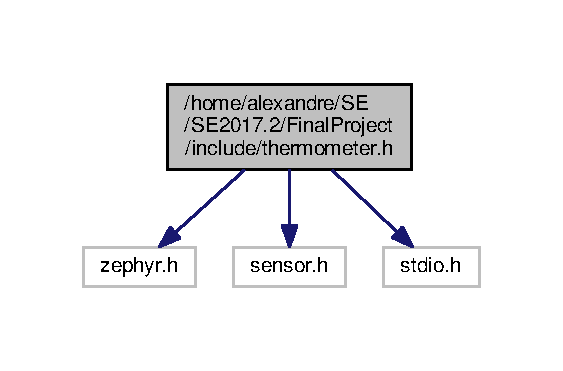
\includegraphics[width=270pt]{thermometer_8h__incl}
\end{center}
\end{figure}
\subsection*{Functions}
\begin{DoxyCompactItemize}
\item 
double \hyperlink{thermometer_8h_a57e729c77b010b0df23c4712905b767c}{thermometer\+\_\+get\+\_\+temperature\+\_\+as\+\_\+double} (void)
\begin{DoxyCompactList}\small\item\em thermometer\+\_\+get\+\_\+temperature\+\_\+as\+\_\+double Read current temperature in celsius from the thermometer device \end{DoxyCompactList}\end{DoxyCompactItemize}


\subsection{Function Documentation}
\index{thermometer.\+h@{thermometer.\+h}!thermometer\+\_\+get\+\_\+temperature\+\_\+as\+\_\+double@{thermometer\+\_\+get\+\_\+temperature\+\_\+as\+\_\+double}}
\index{thermometer\+\_\+get\+\_\+temperature\+\_\+as\+\_\+double@{thermometer\+\_\+get\+\_\+temperature\+\_\+as\+\_\+double}!thermometer.\+h@{thermometer.\+h}}
\subsubsection[{\texorpdfstring{thermometer\+\_\+get\+\_\+temperature\+\_\+as\+\_\+double(void)}{thermometer_get_temperature_as_double(void)}}]{\setlength{\rightskip}{0pt plus 5cm}double thermometer\+\_\+get\+\_\+temperature\+\_\+as\+\_\+double (
\begin{DoxyParamCaption}
\item[{void}]{}
\end{DoxyParamCaption}
)}\hypertarget{thermometer_8h_a57e729c77b010b0df23c4712905b767c}{}\label{thermometer_8h_a57e729c77b010b0df23c4712905b767c}


thermometer\+\_\+get\+\_\+temperature\+\_\+as\+\_\+double Read current temperature in celsius from the thermometer device 

\begin{DoxyReturn}{Returns}
Temperature in celsius 
\end{DoxyReturn}

%--- End generated contents ---

% Index
\backmatter
\newpage
\phantomsection
\clearemptydoublepage
\addcontentsline{toc}{chapter}{Index}
\printindex

\end{document}
